% \documentclass[pdflatex,11pt]{aghdpl}
% \documentclass{aghdpl}               % przy kompilacji programem latex
\documentclass[pdflatex,en]{aghdpl}  % praca w języku angielskim
\usepackage[british,UKenglish,USenglish,english]{babel}
\usepackage[utf8]{inputenc}

\usepackage[backend=bibtex,
%style=numeric,
bibencoding=ascii,
style=alphabetic
%style=reading
]{biblatex}

\addbibresource{bibliografia.bib}

% dodatkowe pakiety
\usepackage{enumerate}
\usepackage{listings}
\usepackage{float}
\usepackage{siunitx}

\lstloadlanguages{TeX}

\lstset{
  literate={ą}{{\k{a}}}1
           {ć}{{\'c}}1
           {ę}{{\k{e}}}1
           {ó}{{\'o}}1
           {ń}{{\'n}}1
           {ł}{{\l{}}}1
           {ś}{{\'s}}1
           {ź}{{\'z}}1
           {ż}{{\.z}}1
           {Ą}{{\k{A}}}1
           {Ć}{{\'C}}1
           {Ę}{{\k{E}}}1
           {Ó}{{\'O}}1
           {Ń}{{\'N}}1
           {Ł}{{\L{}}}1
           {Ś}{{\'S}}1
           {Ź}{{\'Z}}1
           {Ż}{{\.Z}}1
}

\newcommand{\rad}{\radian}

\usepackage{array}
\newcolumntype{L}[1]{>{\raggedright\let\newline\\\arraybackslash\hspace{0pt}}m{#1}}
\newcolumntype{C}[1]{>{\centering\let\newline\\\arraybackslash\hspace{0pt}}m{#1}}
\newcolumntype{R}[1]{>{\raggedleft\let\newline\\\arraybackslash\hspace{0pt}}m{#1}}

\makeatletter
\let\ps@plain\ps@fancy
\makeatother

%---------------------------------------------------------------------------

\author{Grzegorz Gajoch}
\shortauthor{G. Gajoch}

\titlePL{Budowa sensora pochłoniętej dawki promieniowania jonizującego (TID) dla pico-satelitów typu CubeSat}
\titleEN{Total Ionizing Dose (TID) sensor for CubeSat~pico-satellites}

\shorttitlePL{Budowa sensora pochłoniętej dawki promieniowania jonizującego (TID) dla pico-satelitów typu CubeSat} % skrócona wersja tytułu jeśli jest bardzo długi
\shorttitleEN{Total Ionizing Dose (TID) sensor for CubeSat~pico-satellites}

\thesistypePL{Praca inżynierksa}
\thesistypeEN{Bachelor of Science Thesis}

\supervisorPL{dr inż. Cerazy Worek}
\supervisorEN{Cerazy Worek Ph.D}

\date{2016}

\departmentPL{Katedra Elektroniki}
\departmentEN{Department of Electronics}

\facultyPL{Wydział Informatyki, Elektroniki i Telekomunikacji}
\facultyEN{Faculty of Computer Science, Electronics and Telecommunications}

\acknowledgements{Serdecznie dziękuję \dots tu ciąg dalszych podziękowań np. dla promotora, żony, sąsiada itp.}


%---------------------------------------------------------------------------

\begin{document}

\titlepages

\tableofcontents
\clearpage


\chapter{Introduction}

% Introduction

\chapter{Terms, definitions and abbreviated terms}

\section{Abbreviated terms}

\section{Conventions}

% Terms, definitions and abbreviated terms
% - Abbreviated terms
% - Conventions

\chapter{Principles}

\section{Radiation effects on electronic devices}
    There are two basic effects of radiation on silicon components:
    \begin{itemize}
        \item ionizing effect
        \item displacement damage
    \end{itemize}

    Those two effect are responsible for changing parameters of semiconductor devices, which after some time can lead to failure of the device. Main source of this radiation are Gamma (ionization) and Neutron particles (displacement).

    In space electronics during analysis and design two major problems are considered - Single Event Effects (SEE) and Total Ionizing Dose (TID). Every silicon and silica device is susceptible to both of those - and both have to be considered during product design, development and testing.

    \subsection{Single Events Effects}
        Single Event Effects are connected with generation of electron-hole pair in semiconductor, when material is exposed to ionizing radiation. Amount of pairs generated is proportional to energy deposited. For semiconductor device parameter $LET_{th}$ (Linear Energy Transfer Threshold) is defined, being a measure of how susceptible the device is. For particles with Linear Energy Transfer (LET - normalized particle energy per mass of the absorbing material), below this threshold no effect will be observed.

        Single Event Effects are divided into two groups - non-destructive (fully recoverable, possibly after power cycle) and destructive (permanent damage) effects. Shortly those are described below, defined as in \cite{ECSS_Q_ST_60_15C}.

        \bigskip\textbf{Non-destructive effects}
        \begin{itemize}
            \item \textbf{Single Event Upset} - especially memory-based devices (like microprocessors, memories, Field Programmable Gate Array - FPGA) are vulnerable. This phenomenon will possibly alter the state of cell in memory - causing memory corruption. This can lead to complete failure of device if this is not corrected.

            \item \textbf{Single Event Functional Interrupt} - subset of SEU - this effect cause the system to latch in non-recoverable state (e.g. by switching to wrong state in state machine). Only option is to reset circuit to back to known state.

            \item \textbf{Single Event Transient} - are formed as a voltage/current spurious pulses generated by charge induced by striking particle. This can cause different problems - from disturbing analog electronics up to causing switch of digital circuit. This effect strongly depends on size of feature in silica.
        \end{itemize}

        \bigskip\textbf{Destructive effects}
        \begin{itemize}
            \item \textbf{Single Event Latch-up} - particle striking can cause turning on parasitic thyristor in CMOS structure. This will lead to effectively shorting voltage supply to ground, causing overheat and damage to the device.

            \item \textbf{Single Event Gate Rupture} - high energy particle comes through thin gate (especially in MOS transistors) can cause generation of electron-holes pairs in gate and substrate - causing high electric field across gate. When this effect is strong enough it can cause permanent damage to transistor.

            \item \textbf{Single Event Burnout} - ion that traverses the transistor structure (through the source) can induce a current flow that turns on the parasitic npn transistor. This leads to effective short circuit and damage to the device.
        \end{itemize}

        \bigskip\textbf{Mitigation techniques}

        Below recommended mitigation techniques for SEE were listed:
        \begin{itemize}
            \item SEU - redundancy, memory scrubbing,
            \item SEFI - watchdog, proper reset sequence,
            \item SET - use lower-integration scale devices, implement protection resistors etc.
            \item SEL - implement overcurrent circuits (like Latch-up Current Limiters),
            \item SEGR, SEB - use higher $LET_{th}$ devices
        \end{itemize}

    \subsection{Total Ionizing Dose}
        TID is defined as total energy absorbed during exposure. This can be caused by any kind of radiation, behaving differently in every semiconductor device. In general, TID successively degrades electronic device parameters in time, causing them to stop functioning when critical irradiation was reached. Effect in p-MOSFET transistor is described in section \ref{Radiation_effects_on_MOS_transistors}.

        Every qualified device for spacecraft system will have tested value of TID value, for example by MIL-STD-883G, Test Method 1019.7 \cite{MIL_STD_883}. For example, ADC128S102QML-SP have a guaranteed value of 100 kRad.

\section{Need for TID radiation dosimetry}
    During spacecraft mission accumulated radiation level should be monitored to not excess guaranteed values for components. For example, near end of its lifetime, spacecraft can be commanded to deorbit into atmosphere or move to parking orbit - before fail can occur, causing losing control of spacecraft.
    Absorbed dose simulation and estimation is possible, but results are averaged by long period of time. Constantly flying by South Atlantic Anomaly or Van Allen belts can cause radiation estimation to be inaccurate, so near all spacecrafts implement sensor which constantly monitor radiation level absorbed by its electronics.

\section{On-line TID radiation dosimetry}

\section{RadFET Theory}

    \subsection{Radiation effects on MOS transistors}
    \label{Radiation_effects_on_MOS_transistors}

    \subsection{Threshold voltage measurement}

    \subsection{Temperature dependencies}

% Principles
% - Ionising radiation
% - Radiation effects on electronics
% -- Single Events Effects
% -- Total Ionising Dose
% - Need for TID radiation dosimetry
% - On-line TID radiation dosimetry
% - RadFET Theory
% -- Radiation effects on MOS transistors
% -- Threshold voltage measurement
% -- Temperature dependencies

\chapter{Design requirements}

In this chapter the requirement for the TID sensor will be presented.

Sensor is designed to be flown on-board of PW-Sat2 satellite. Therefore it should be designed for its particular requirements. In addition, it should be designed having in mind active space standard and launcher requirements.


\section{PW-Sat2}
    Presented sensor is scheduled to be launched on PW-Sat2 satellite \cite{PW-Sat2URL}. Therefore it should be designed especially for this particular type of mission. In this section PW-Sat2 mission will be presented. 

    On fig. \ref{PW-Sat_render_01} exploded render of PW-sat2 is presented.

    \begin{figure}[h]
        \centering
        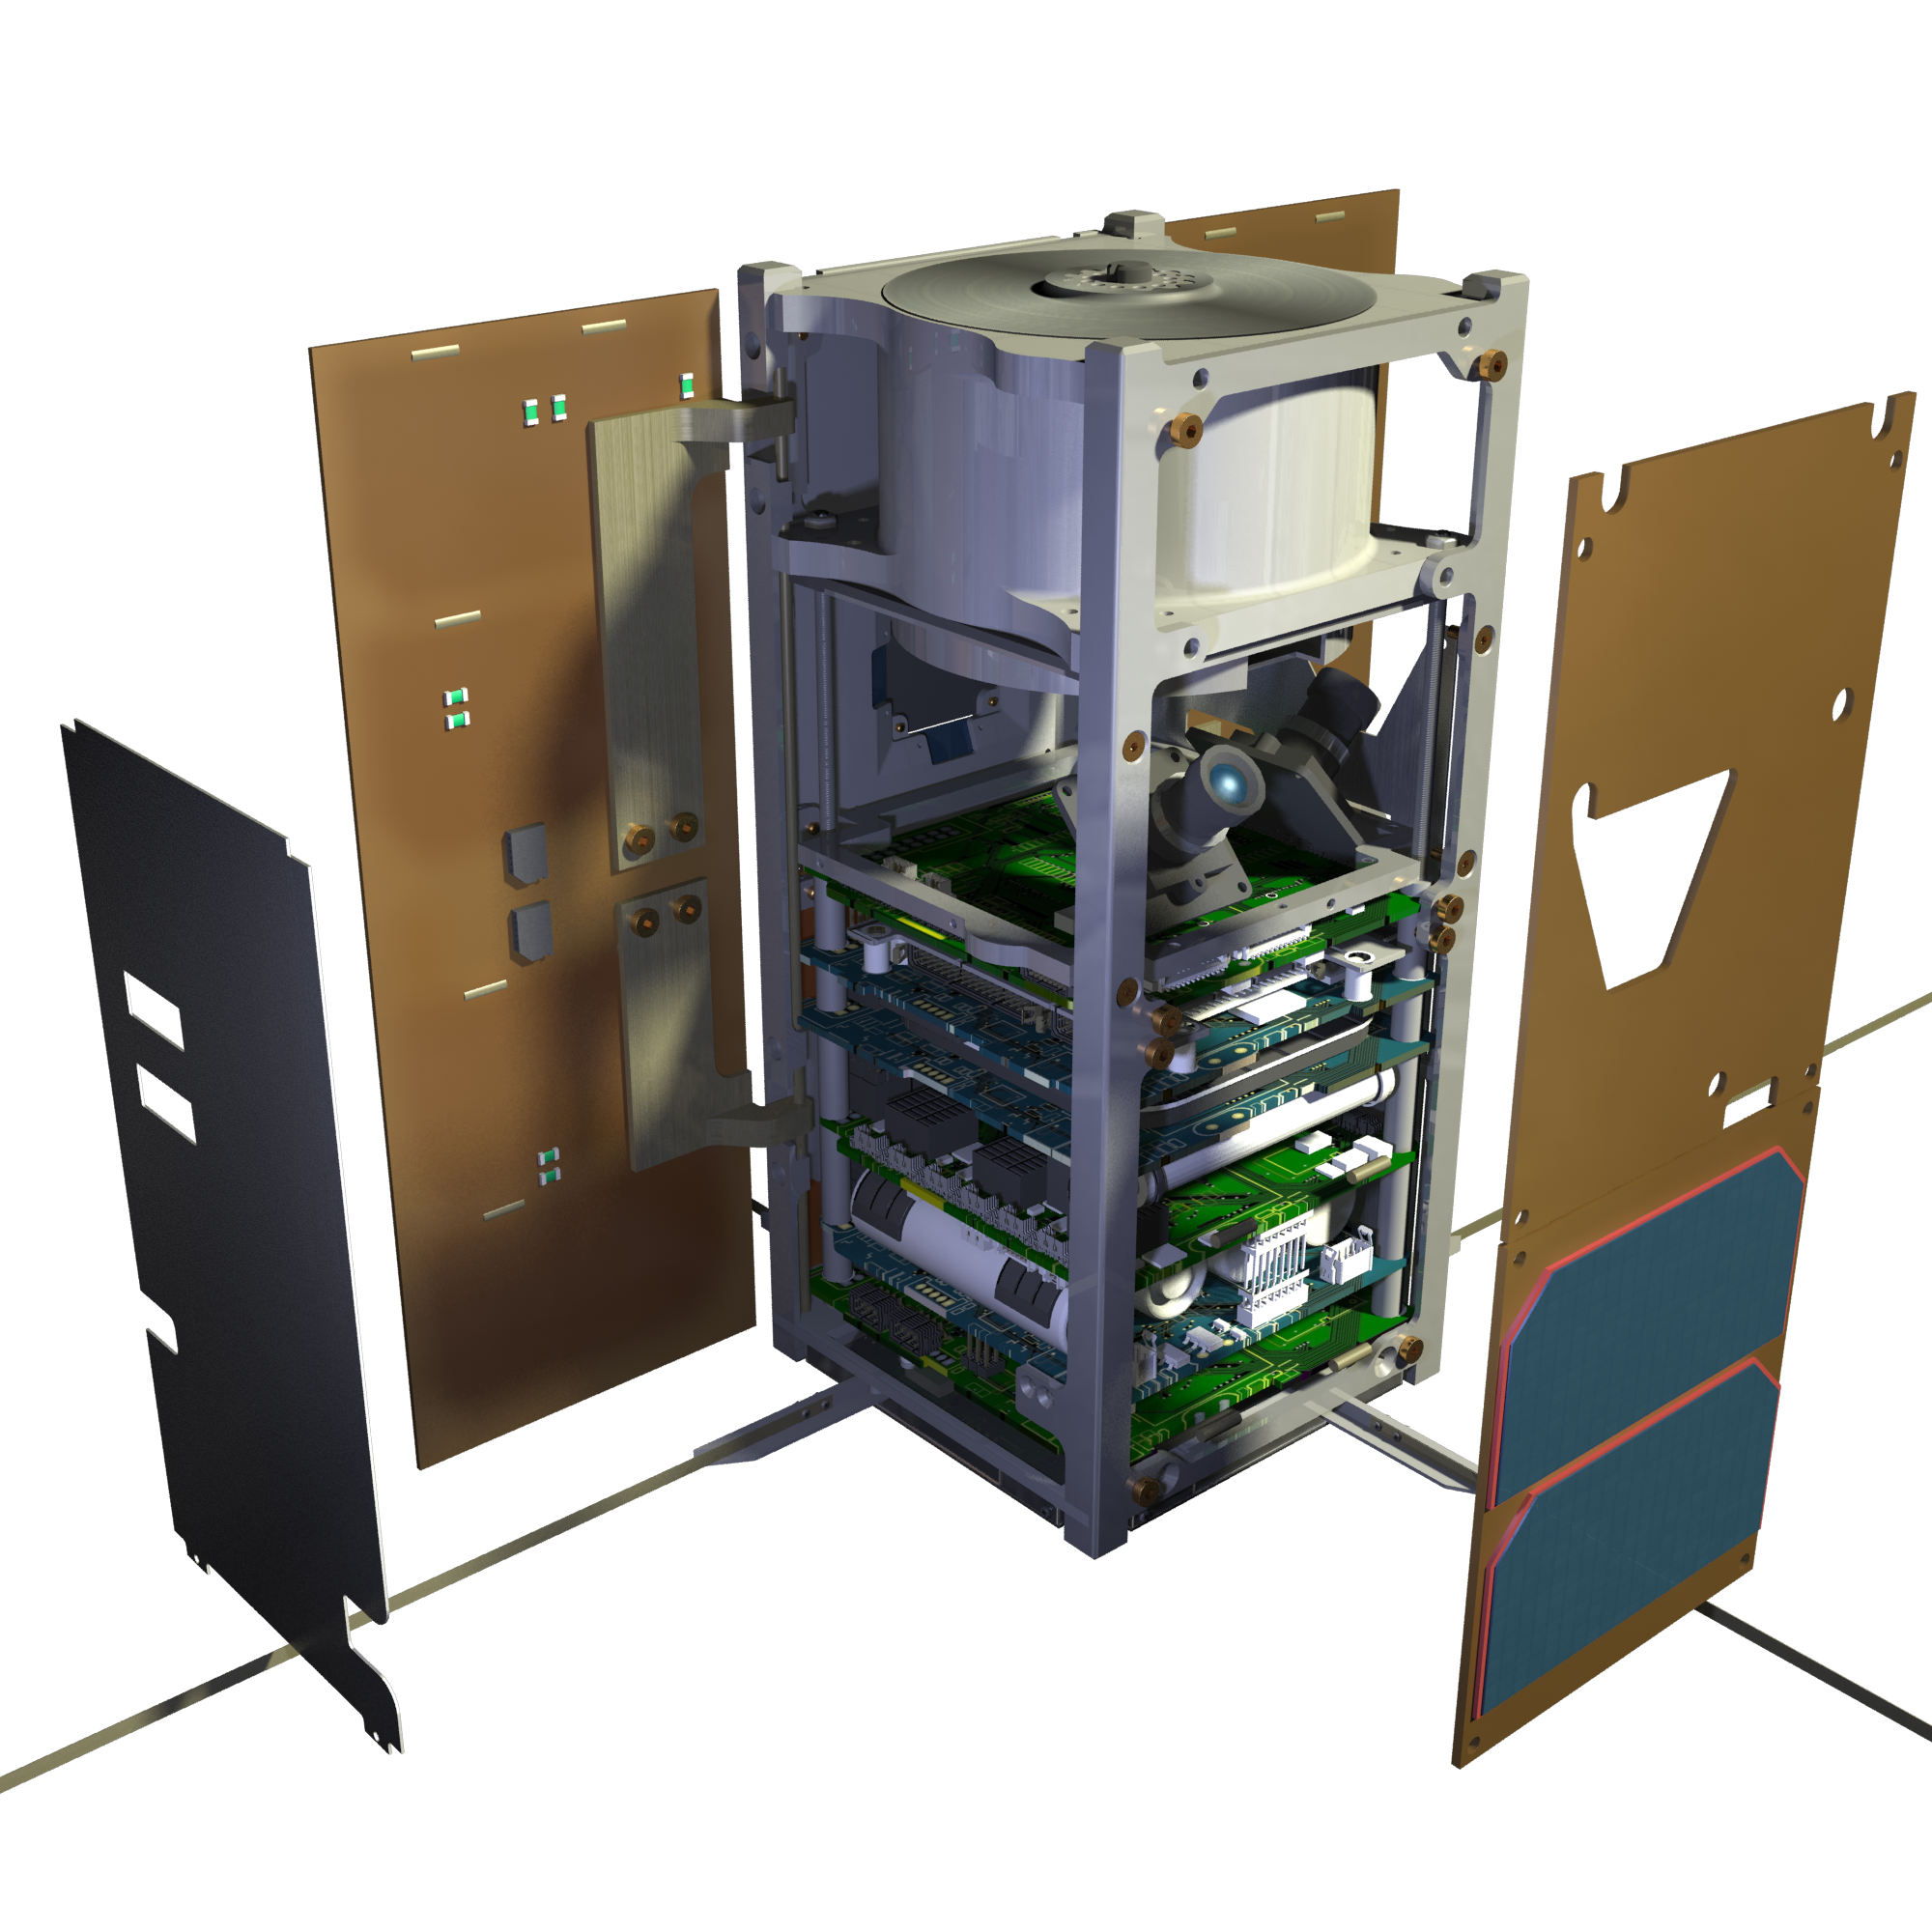
\includegraphics[width=0.5\paperwidth]{img/PW-Sat2_render_01.png}
        \caption{PW-Sat2 render (by M. Świetlik)}
        \label{PW-Sat_render_01}
    \end{figure}

    PW-Sat2 is scheduled to be launched on Falon9 rocket from SpaceX company in Q4 2017.

    \begin{figure}[H]
        \centering
           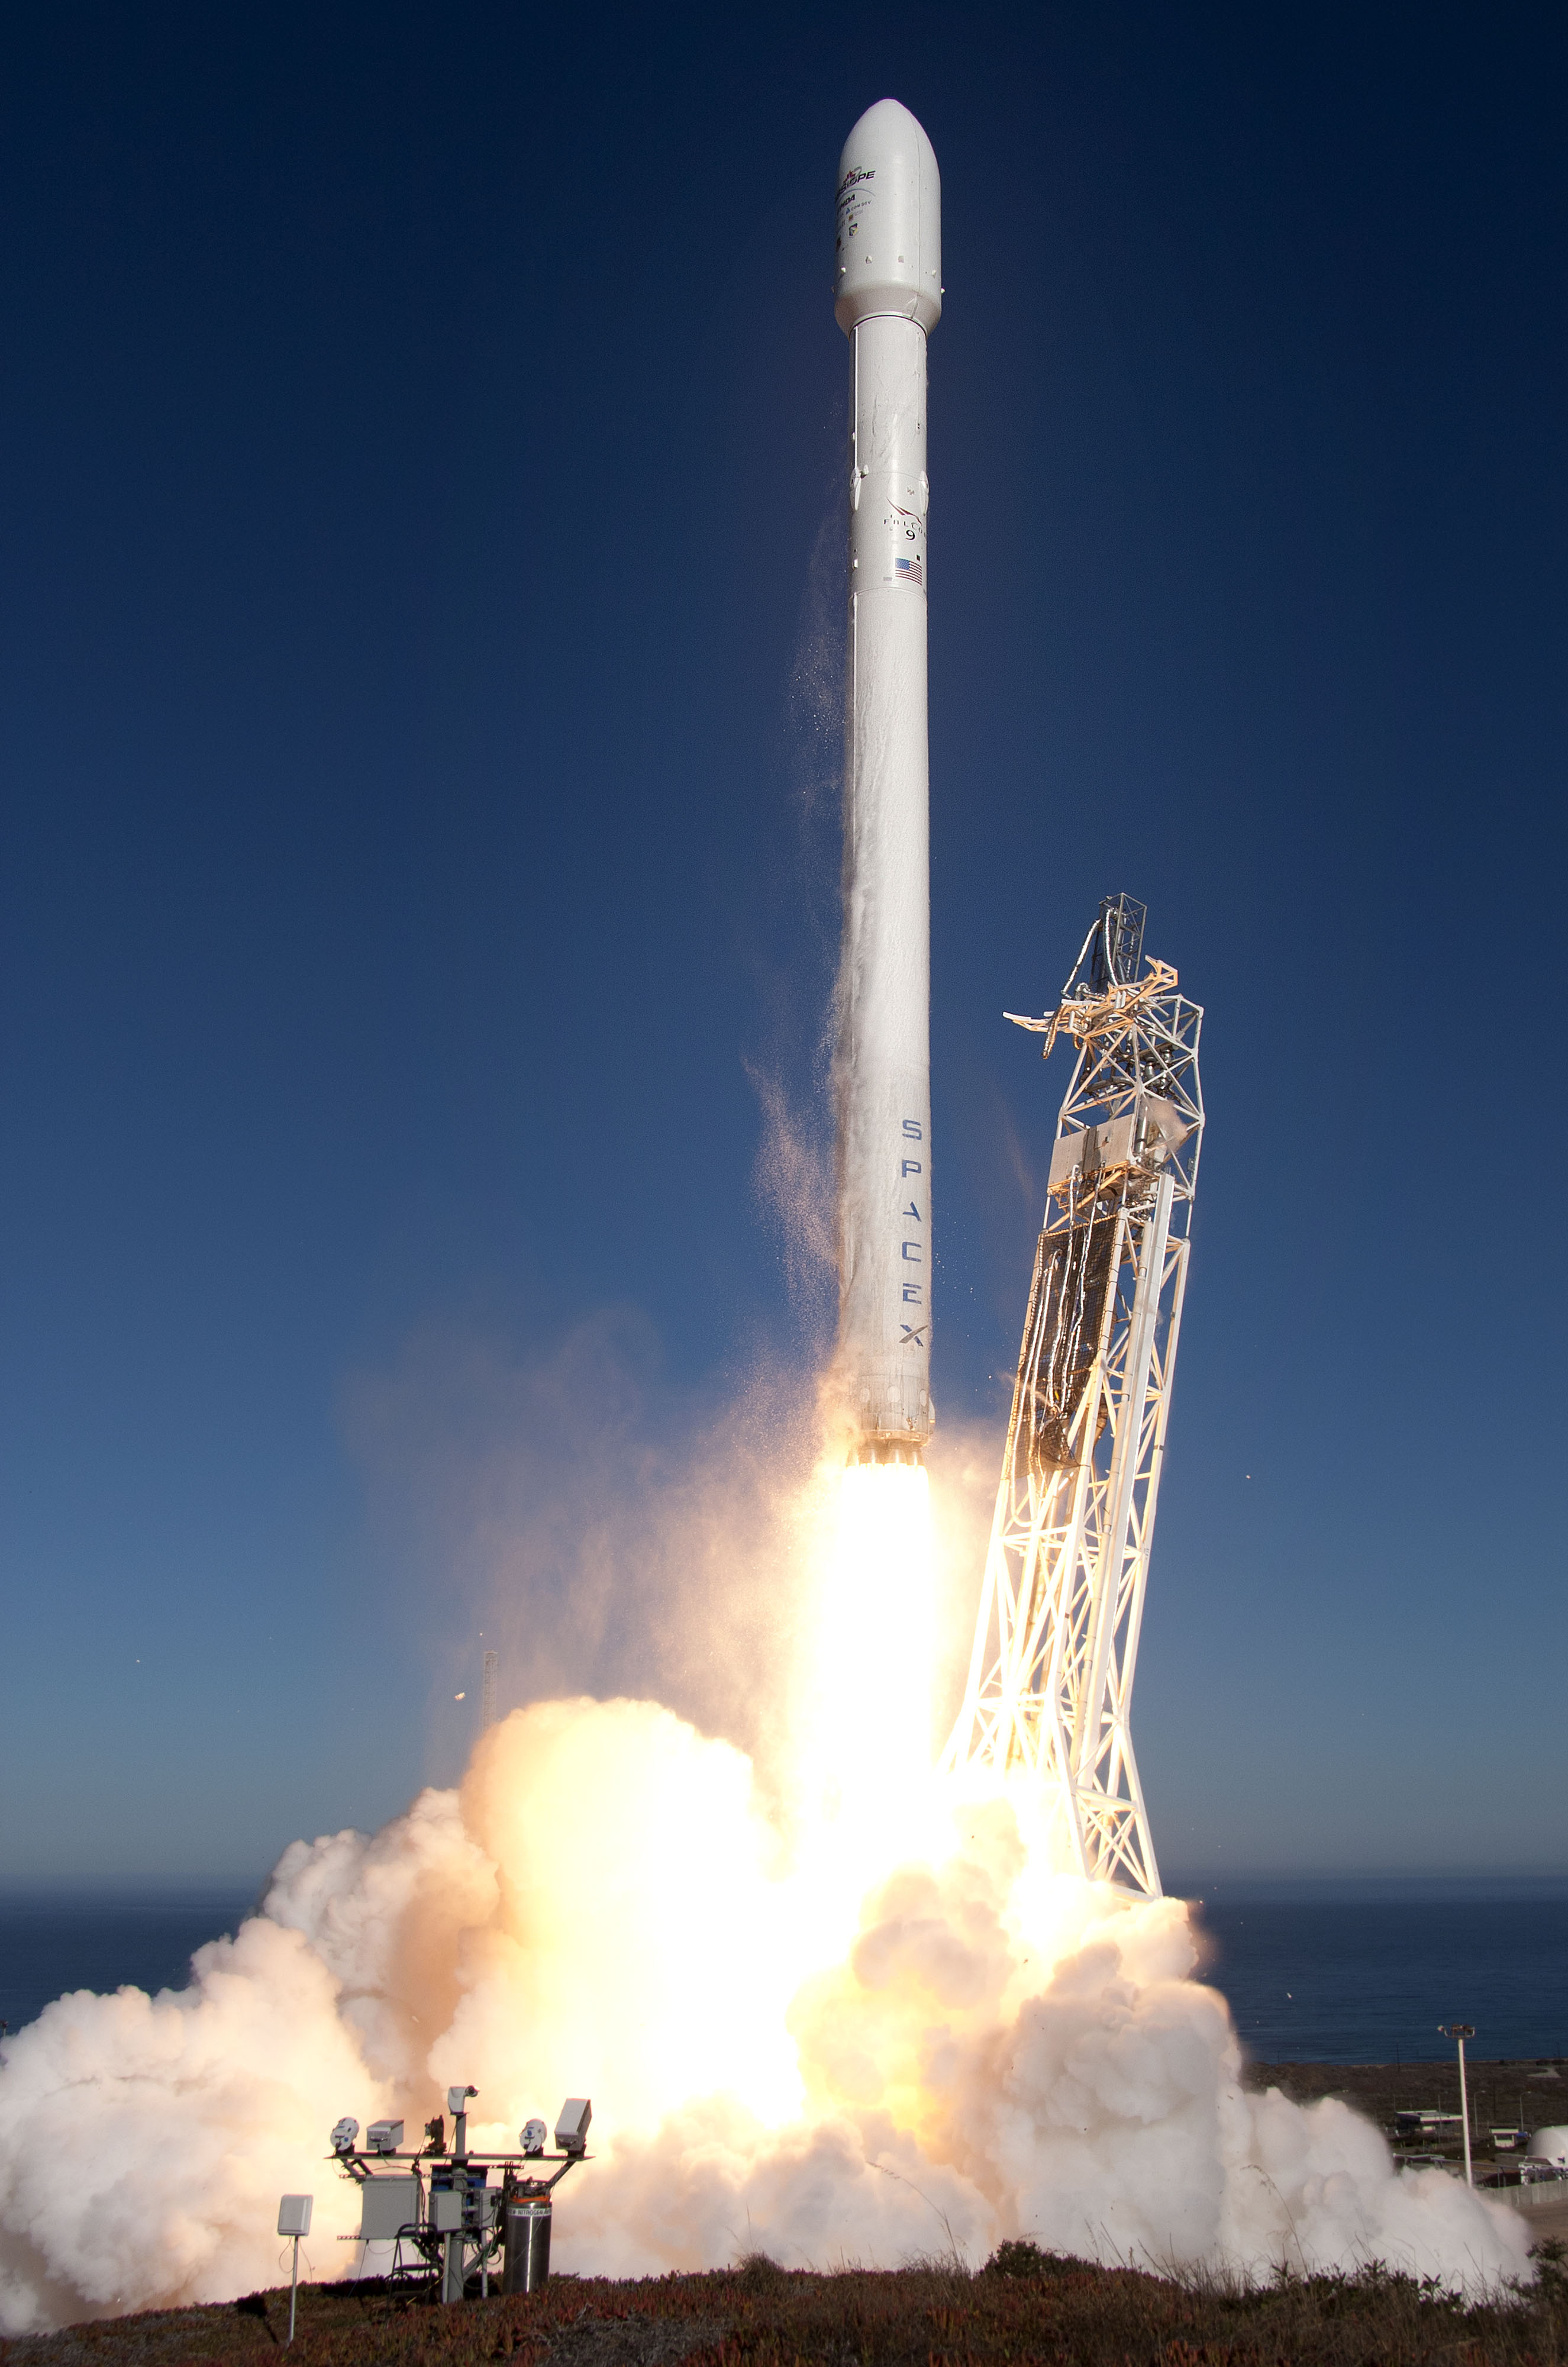
\includegraphics[width=0.3\paperwidth]{img/Falcon9.jpg}
        \caption{Falcon9 rocket. Source: \url{www.spacex.com}}
        \label{PW-Sat_render_01}
    \end{figure}


\subsection{Primary mission}
    Primary mission of PW-Sat2 is to test deorbit sail. Its purpose is to increase atmospheric drag and shorten satellite life. This method of deorbitation could be easy way to reduce space debris on LEO. Render of PW-Sat2 with opened sail is on \ref{PW-Sat_render_sail}.

    \begin{figure}[H]
        \centering
        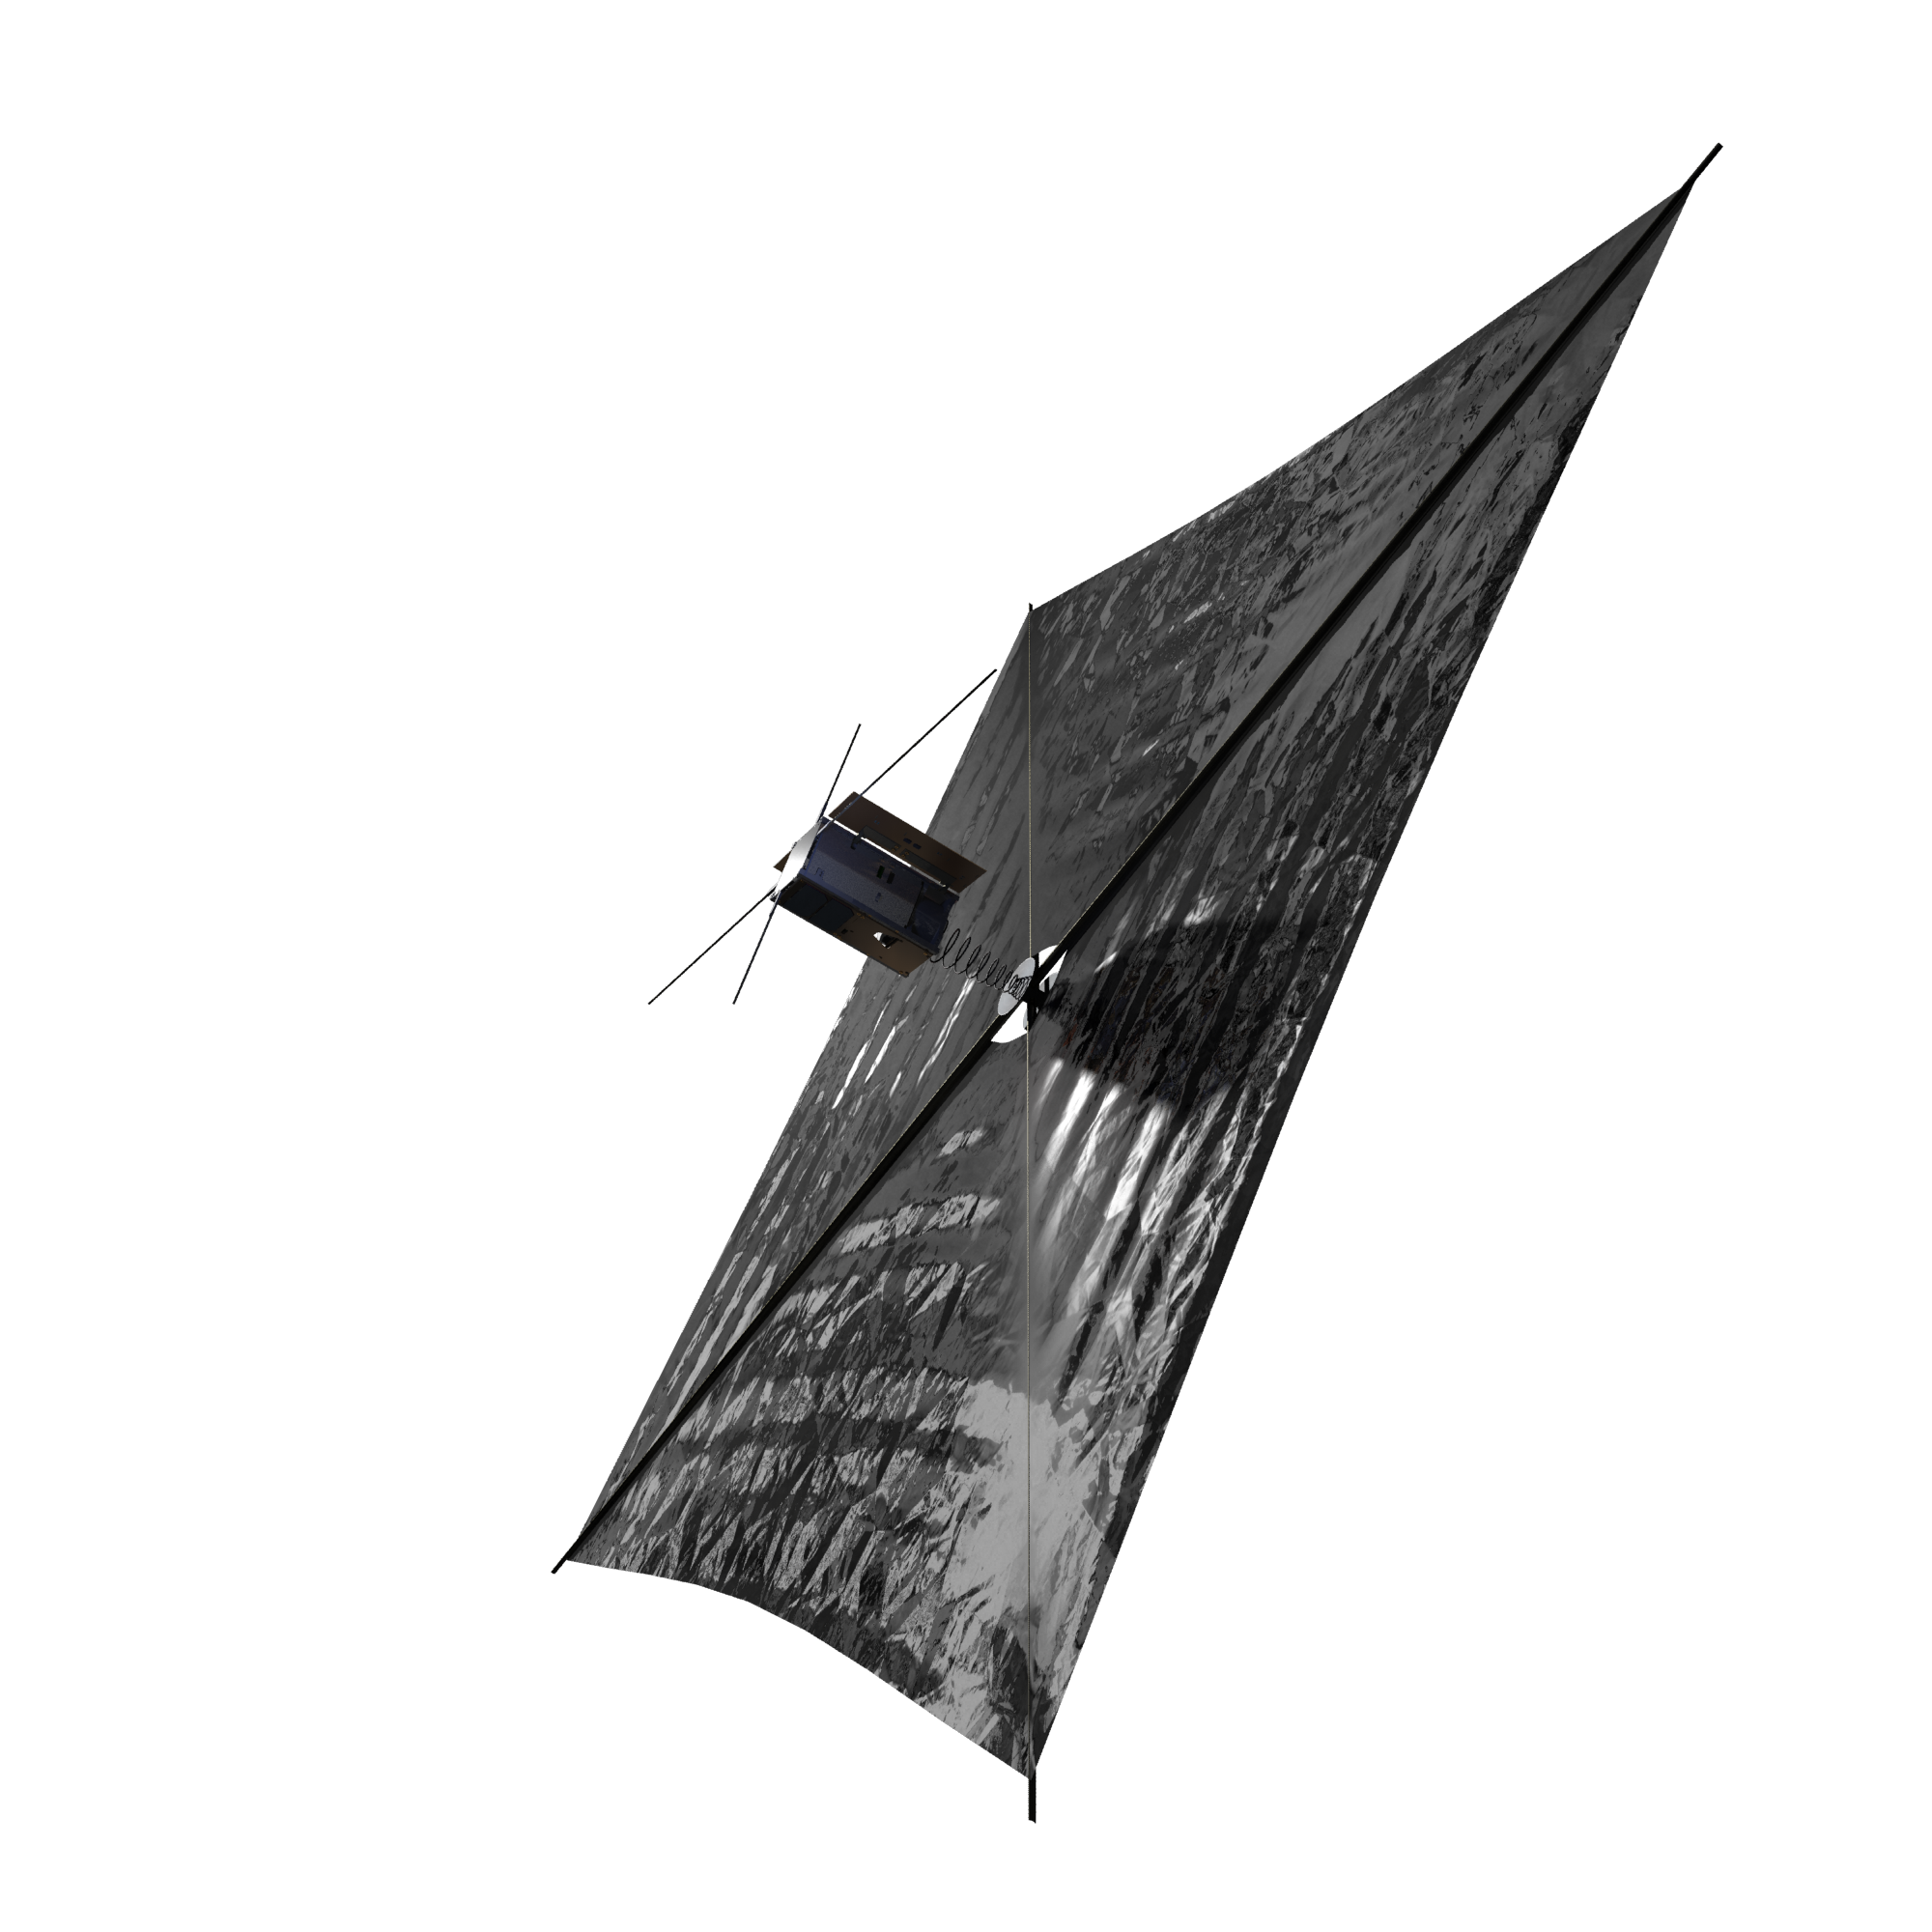
\includegraphics[width=0.7\paperwidth]{img/PW-Sat2_render_02.png}
        \caption{PW-Sat2 with opened sail (by M. Świetlik)}
        \label{PW-Sat_render_sail}
    \end{figure}

    More information about this experiment can be found in \cite{DDC_article}.

\subsection{Lifetime}
    Due to its primary mission PW-Sat2 lifetime is planned to be 40 days long. After this time deorbit sail will open, and orbit will slowly decrease. Deorbitation from nominal orbit is planned to take N days. Therefore sensor should be able to measure dose absorbed during full mission - N days.

\subsection{Orbit}
    PW-Sat2 in planned to be launched to sun-synchronous circular orbit of attitude \SI{575}{\kilo\meter}, with LTAN of $10:30$ \cite{PWSAT_MA_CDR}.


\subsection{Radiation analysis}
    Simulations in SPENVIS \cite{SPENVIS_URL} were performed to estimate TID accumulated during PW-Sat2 mission. On fig \ref{TIDvsSheilding} dose as a function of shielding thickness was plotted.

    \begin{figure}[H]
        \centering
        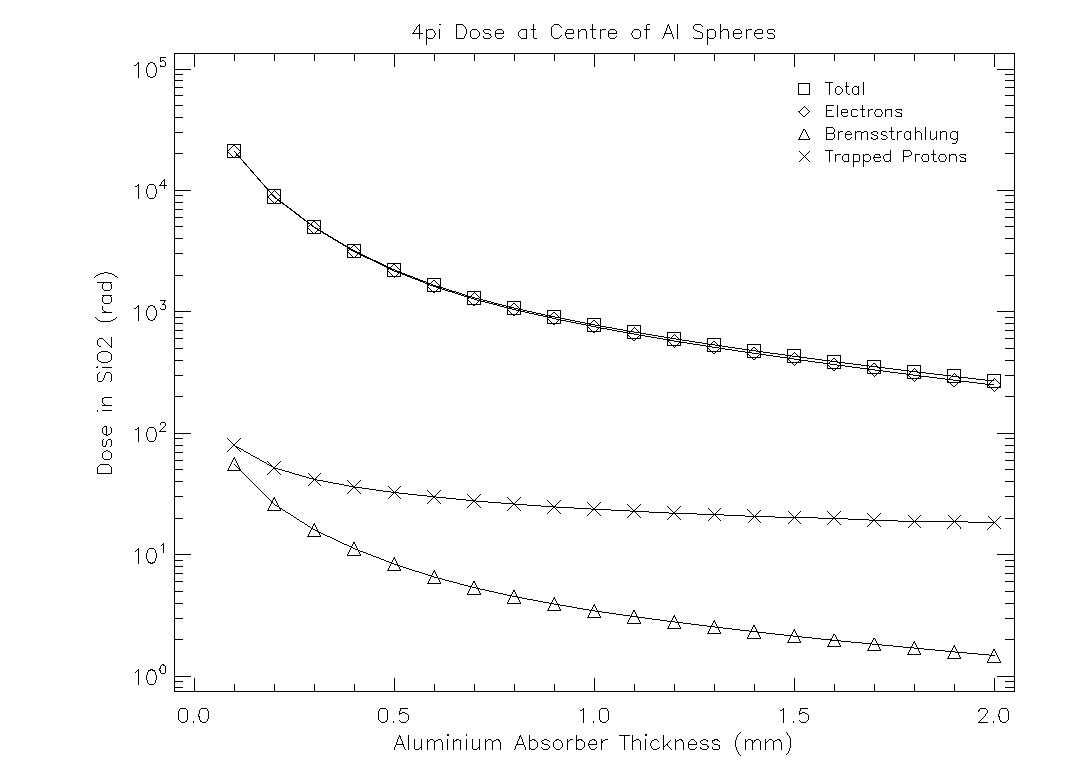
\includegraphics[width=0.7\paperwidth]{img/dose.eps}
        \caption{TID vs shielding}
        \label{TIDvsSheilding}
    \end{figure}

    Shielding of PW-Sat2 is about \SI{0.5}{\milli\meter} thick (aluminum sides as well as aluminum substrate for solar cells - \ref{PW-Sat_render_01}). Therefore predicted dose during PW-Sat2 mission is about \SI{10}{\kilo\rad}.


\section{Sensor requirements}
    Summing PW-Sat2 mission analysis, high-level sensor requirements were estimated:

    \begin{itemize}
        \item Total range of the sensor should be more than predicted dose. Derating this value gives range of about \SI{3}{\kilo\rad}.

        \item Resolution should be lower than \SI{0.1}{\kilo\rad}, 

        \item Total accuracy (across temperature \& component aging) should be less than \SI{0.5}{\kilo\rad}.
    \end{itemize}




\section{Applicable standards}
    The sensor should comply to ECSS \cite{ECSS_URL} standards. They are required by launch provider, as well as describing good practices during space product development.

    ESCIES \cite{ESCIES_URL} provide valuable knowledge about components qualifications, testing and verification.



\section{Electrical requirements}
    Sensor will be placed on-board of PW-Sat2. Therefore it should comply to its' standards - power supplies, communication interfaces etc.

\subsection{Electronics stack}
    Modules on PW-Sat2 are connected in PC-104 stack structure as shown on figure \ref{PW-Sat2_stack}. Is is placed inside structure and consists of (from the top):
    \begin{itemize}
        \item Payload module (PLD)
        \item On-Board Computer (OBC)
        \item Attitude Determination and Control Subsystem (ADCS)
        \item Electrical Power System (EPS)
        \item battery module (ACC)
        \item communication transceiver (COMM)
        \item antennas module (ANT)
    \end{itemize}

    \begin{figure}[H]
        \centering
        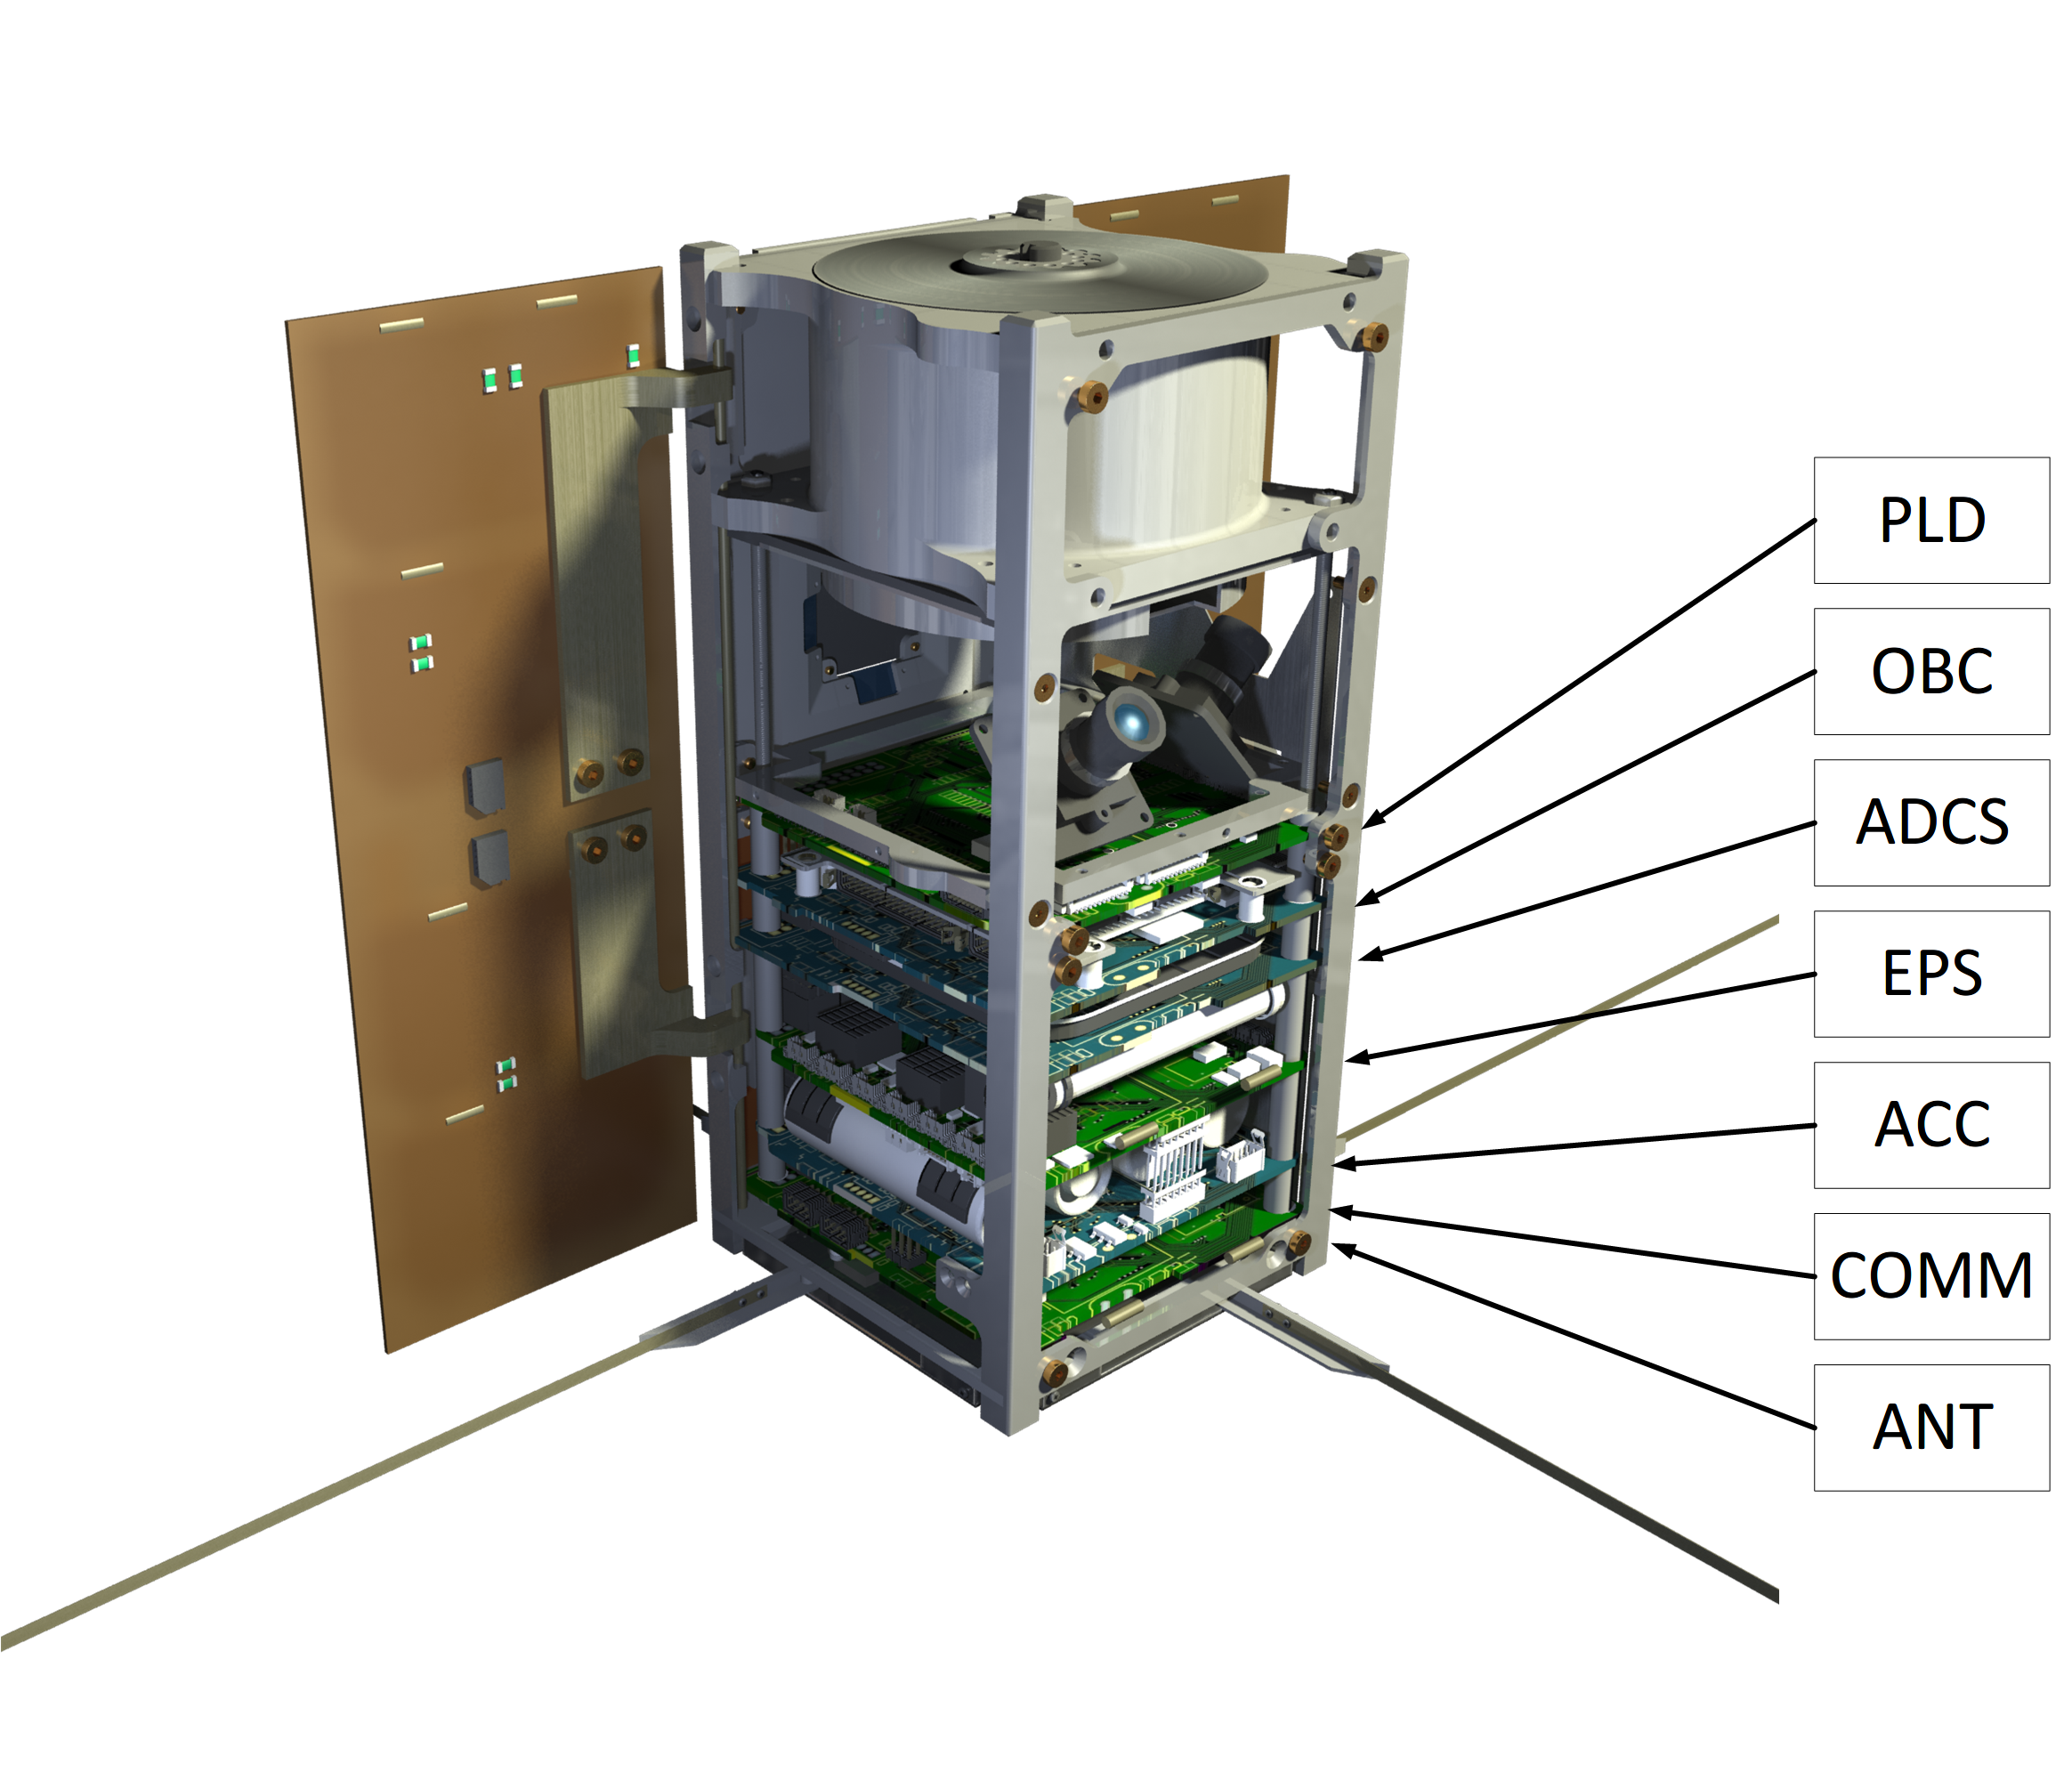
\includegraphics[width=0.7\paperwidth]{img/PW-Sat2-stack.png}
        \caption{PW-Sat2 electronics stack}
        \label{PW-Sat2_stack}
    \end{figure}


    Sensor will be placed on Payload board, on the top of PC-104 stack. It will be placed on its PCB, described in \ref{PCB_description}. It will be one of sensors on this board, connected to PC-104 stack.


\subsection{PC-104 connector}
    PLD board is connected to OBC with PC-104 connector. Pinout is shown on figure \ref{PC104_PLD}.

    \begin{figure}[H]
        \centering
        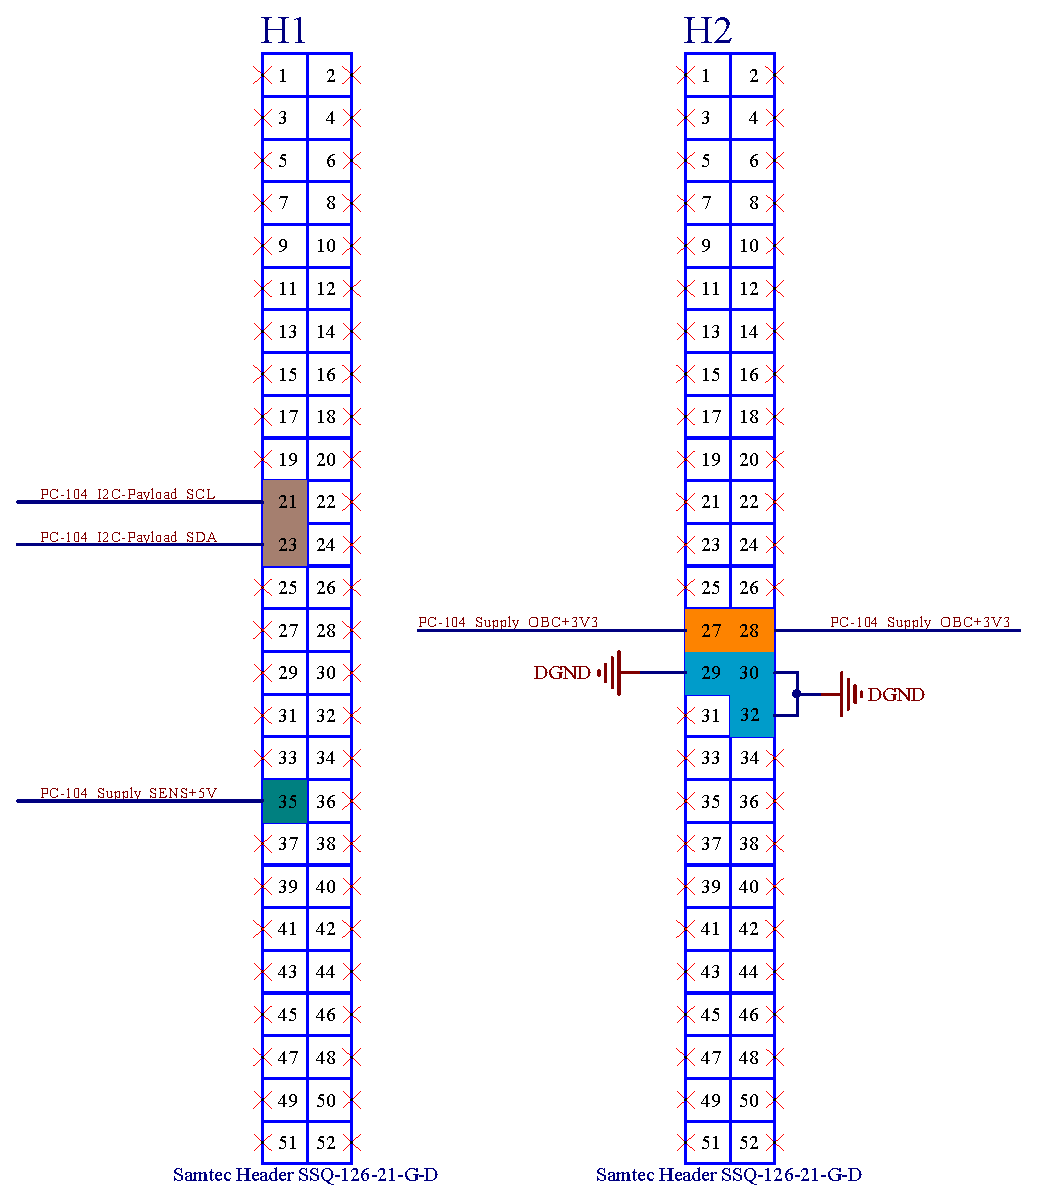
\includegraphics[width=0.5\paperwidth]{img/PC-104.eps}
        \caption{PC-104 connector to PLD board}
        \label{PC104_PLD}
    \end{figure}

    Connector consists of:
    \begin{itemize}
        \item $I^2C$ bus, connected directly to MCU on OBC
        \item SENS \SI{5}{\volt} line, powered when sensor is enabled by OBC
    \end{itemize}

\subsection{Power rail}
    As mentioned earlier, the power for the sensor is \SI{+5}{\volt}, activated whenever sensor should be accessed by OBC. 

    Power line is controlled and protected by Latchup-Current Limiter FPF2701MX placed on EPS board. Therefore additional latchup protection in not necessary in this design. However, this sensor will be not only one on PLD board and should have it's own power switch. PLD board is enabled and disabled by EPS on OBC command and sensor should be enabled only during TID readout. Having this in mind forces the design to be immune to immediate shutdowns. 

\subsection{Power consumption}
    During irradiation sensor should be completely turned off. It decreases possibility of radiation damage and increases overall system reliability.

    During readout required power should be less than \SI{1}{W}.

\subsection{Data interface}
    The sensor is connected to OBC via $I^2C$ interface. OBC on this bus is master - and sensor should be one of slaves. PLD board can be disabled, therefore it should provide isolation of $I^2C$ bus when it is powered off.

\subsection{Radiation immunity}
    Design should be itself immune to radiation. For PW-Sat2 threshold of \SI{10}{\kilo\rad} was chosen for all COTS components. Semiconductor components should have radiation as described in \cite{ESCIES_TID_test_method}.

\subsection{Electromagnetic compatibility}
    EMC requirements are described in \cite{ECSS_E_ST_20_07C}. This standard was tailored to PW-Sat2 because power rail is \SI{+5}{\volt}, other than on bigger S/C (\SI{+28}{\volt}).

    \begin{itemize}
        \item Conducted susceptibility is shown on figure \ref{EMC_conducted_susceptibility} . It was created by down-scaling figure A-4 from \cite{ECSS_E_ST_20_07C} by factor of $\SI{28}{\volt}/\SI{5}{\volt} = 5.6$. EMC limit on power line is defined as constant \SI{175}{\milli\volt} from \SI{30}{\hertz} to \SI{100}{\kilo\hertz}. Sensor should be able to filter this ripple to produce stable power for analog devices. In addition, it should be taken into account that output DC-DC converters on EPS runs on \SI{500}{\kilo\hertz}.

        \begin{figure}[H]
            \centering
            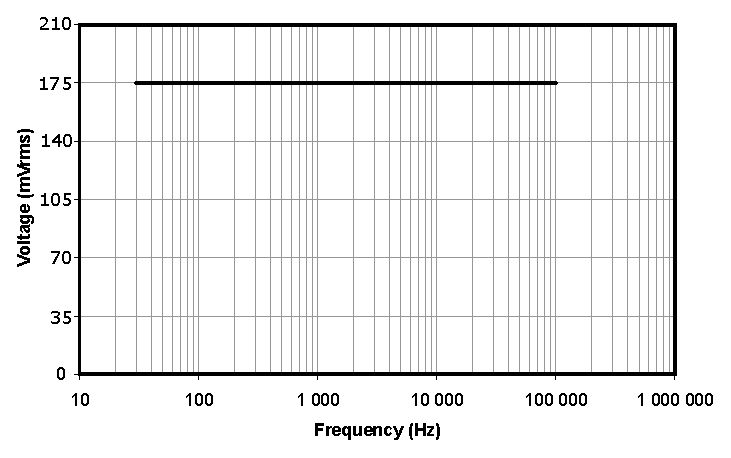
\includegraphics[width=0.5\paperwidth]{img/EMC_conducted_susceptibility.eps}
            \caption{Conducted susceptibility limit, frequency domain. Source: \cite{ECSS_E_ST_20_07C}}
            \label{EMC_conducted_susceptibility}
        \end{figure}


        \item Conducted emission is defined on figure \ref{EMC_conducted_emission}.

        \begin{figure}[H]
            \centering
            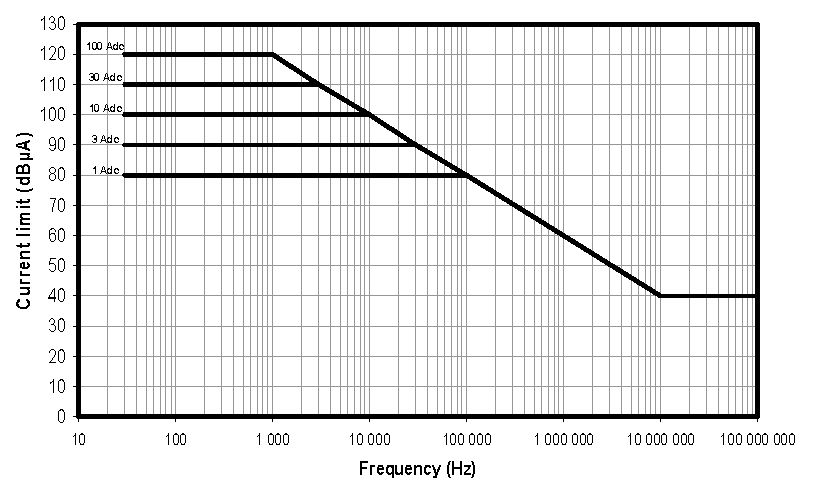
\includegraphics[width=0.5\paperwidth]{img/EMC_conducted_emission.eps}
            \caption{Conducted susceptibility limit, frequency domain. Source: \cite{ECSS_E_ST_20_07C}}
            \label{EMC_conducted_emission}
        \end{figure}    


        \item Radiated susceptibility.
            On board PW-Sat2 is a communication module transmitting \SI{0.5}{\watt} of power on frequency \SI{435.02}{\mega\hertz}. It is planned that during readout radio transmitter will be disabled, but proper tests should be conducted to check for possible errors and faults.

            PLD board is placed near OBC - so radiated emission from digital lines can couple to sensor elements causing noise and errors. Proper tests will be conducted and if necessary shielding will be implemented.

        \item Radiated emission.
            Sensor is not predicted to emit any kind of radio waves. In case of detected anomaly further design decisions would have to be made.

    \end{itemize}


\subsection{Inrush current}
    Inrush current have to be limited to maximum power consumption to not trigger LCL on EPS.

\subsection{Reliability of components}
    This sensor is not a critical part of the satellite. But, reliable components should be used to ensure proper results. 

    Every used component should have failure rate of $0.1\si{\percent}$ or lower. This is essential in capacitors and other passive components.


\section{Mechanical requirements}
    In this chapter design constrains and mechanical requirements of Falcon9 are presented. Launcher requirements were taken from \cite{Falcon9_user_manual}.

\subsection{PCB}
\label{PCB_description}
    PCB of PLD board is standard 4-layer FR4 board with stack shown on figure \ref{PLD_PCB_stack}. Its dimensions are shown on \ref{PLD_PCB_size}, but design is forced to take much less space. For this sensor limits are \SI{3x3}{\centi\meter} double sided.

    \begin{figure}[H]
        \centering
        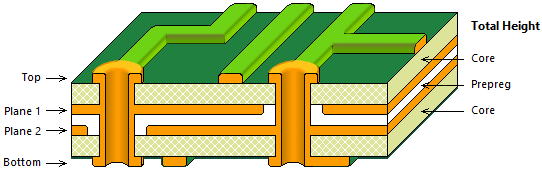
\includegraphics[width=0.5\paperwidth]{img/PLD_PCB_stack.png}
        \caption{PLD board PCB stack}
        \label{PLD_PCB_stack}
    \end{figure}    

    \begin{figure}[H]
        \centering
        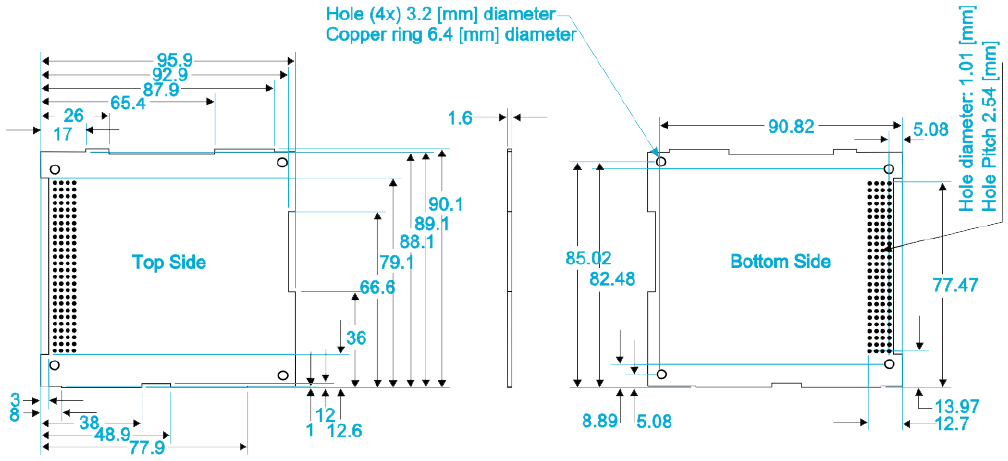
\includegraphics[width=0.7\paperwidth]{img/PC104_PLD_size.png}
        \caption{PC-104 size}
        \label{PLD_PCB_size}
    \end{figure}    



\subsection{Outgassing}
    Every used component should be able to work in vacuum. Outgassing of components should be known to conduct required vacuum tests before launch.

\subsection{Vibration}
    During rocket launch large vibrations occur on payload, therefore it should be immune to it. In case of any heavy electronic components appropriate glue should be applied to prevent joint cracks.
    \begin{figure}[H]
        \centering
        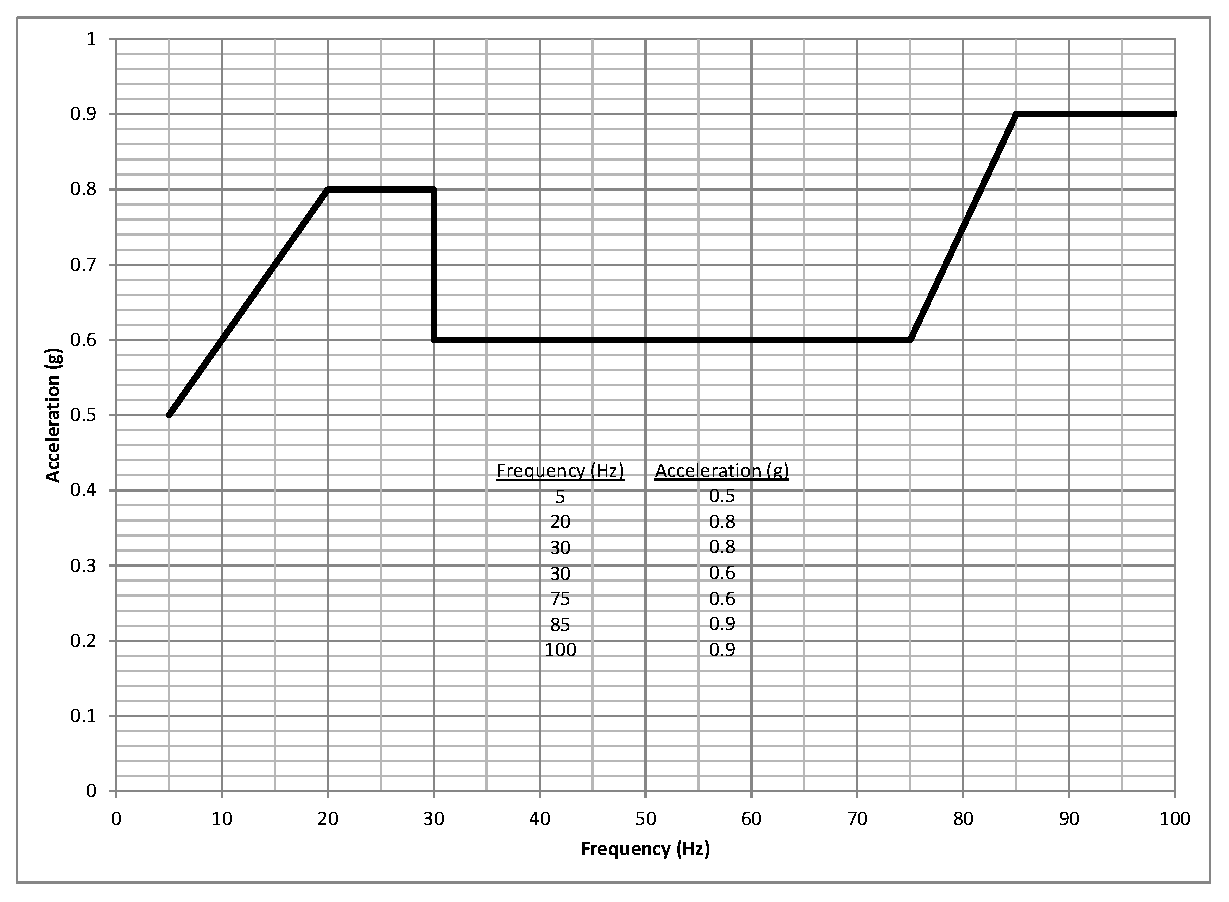
\includegraphics[width=0.5\paperwidth]{img/Falcon9_vibration.eps}
        \caption{Falcon9 maximum axial equivalent sine environment. Source: \cite{Falcon9_user_manual}}
        \label{Falcon9_vibration}
    \end{figure}    


\subsection{Operation temperature}
    The sensor should work in every operational case satellite can be. Simulations were performed to find bounds of possible temperature range inside satellite.    In \cite{PWSAT_TCS_CDR} results are presented. 

    For PLD board operation range is $\SI{0}{\degreeCelsius}$ to $\SI{60}{\degreeCelsius}$. If the measured temperature will be outside this region, sensor will not be enabled.


\subsection{Thermal cycles}
    Or PW-Sat2 orbit sun illumination is changing every $\approx \SI{90}{\minute}$. Therefore large number of thermal cycles are applied to On-Board electronics, which can cause joint cracks as well as component failures. Proper soldering and component selection will be made, according to ECSS.

    As described in \cite{ECSS_Q_ST_70_04C} the sensor should pass thermal cycle tests: $100$ times from $- (100 \pm 5)$\si{\degreeCelsius} to $(100 \pm 5)$\si{\degreeCelsius} in vacuum environment. Test procedure is shown on \ref{thermal_tests}.

    \begin{figure}[H]
        \centering
        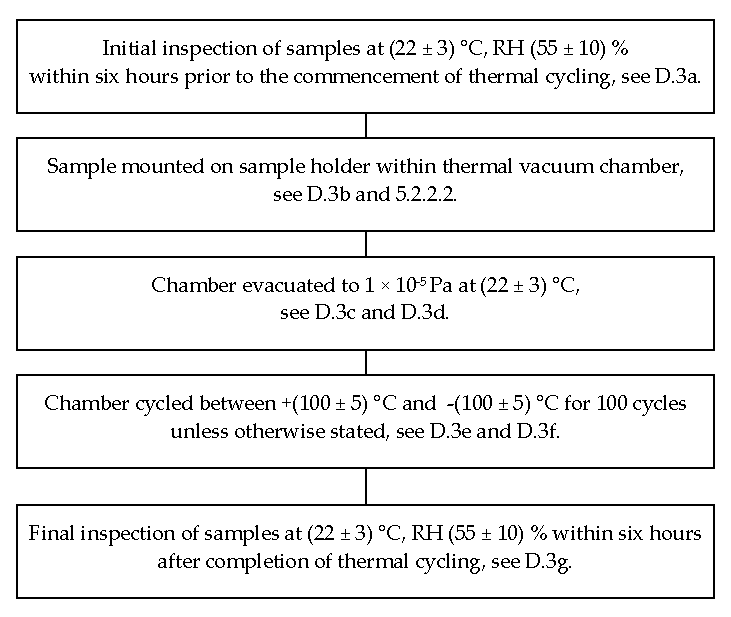
\includegraphics[width=0.5\paperwidth]{img/thermal_cycles.eps}
        \caption{Thermal cycles test procedure. Source: \cite{ECSS_Q_ST_70_04C}}
        \label{thermal_tests}
    \end{figure}

% Design requirements
% - Sensor requirements
% -- Required sensitivity
% -- Required accuracy
% - Applicable standards
% - PW-Sat Mission
% -- Main purpose
% -- Orbit \& lifetime
% -- Radiation analysis
% - Electrical requirements
% -- Electronics stack
% -- Power
% -- Data interface
% -- Radiation immunity
% -- Reliability of components
% - Mechanical requirements
% -- PCB stack \& PCB restrictions
% -- Space available
% -- Vibration
% -- Operation temperature
% -- Thermal cycles

\chapter{Sensor design}
This chapter will cover sensor basics, sensing element selection and theory of operation. The design will be presented at a system-level view. For a more detailed description of the electronics, please skip to chapter \ref{Engineering_model_chapter}.

\section{Review of commercially available RadFETs}
    Commercial solutions are based on a modified MOS structure (with thicker gate region). Example silicon structure is shown in the figure \ref{Tyndall_radfet_silicon}. Different companies produce their own RadFET devices, by designing individual structures fitted to particular requirements. Researched companies only produce the RadFET sensors, leaving the readout circuit design for the customer to realise. A physical schematic and description for RadFET sensors is found in section \ref{Radiation_effects_on_MOS_transistors}. In the table \ref{commercial_radfet_comparison} commercially available RadFETs are compared.

    \begin{figure}[H]
        \centering
        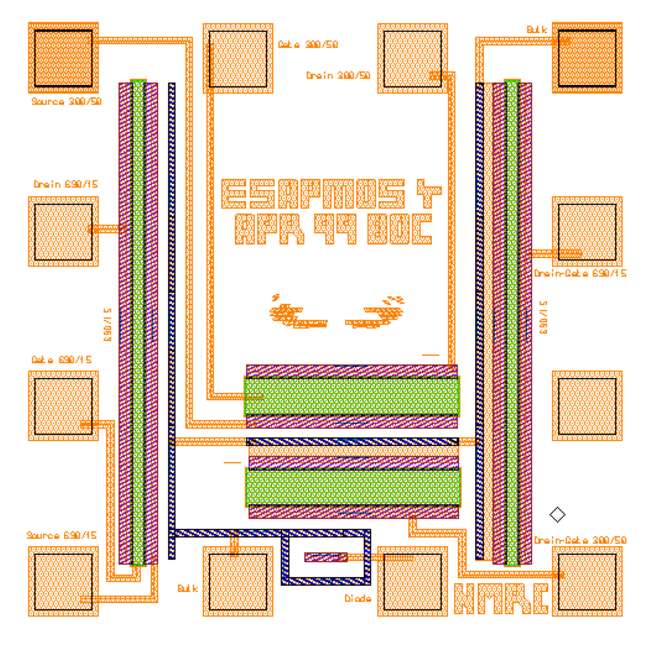
\includegraphics[width=0.45\paperwidth]{img/05/radfet-silicon.eps}
        \caption{4x RadFET silicon structure by Tyndall. Source: \cite{Tyndall_Radfet}}
        \label{Tyndall_radfet_silicon}
    \end{figure}

    \begin{table}[H]
    \caption{Commercial RadFET comparison}
    \label{commercial_radfet_comparison}
    \begin{tabular}{| L{3.5cm} | C{3.5cm} | C{3.5cm} | C{3.5cm} |}
        \hline
        Type: & REM RFT300 & Tyndall TY1003 & Tyndall TY1004 \\ \hline

        Image: &
        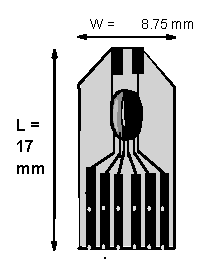
\includegraphics[width=0.10\paperwidth]{img/05/rem.eps} &
        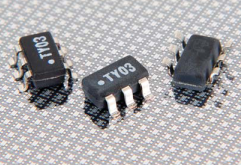
\includegraphics[width=0.15\paperwidth]{img/05/TY1003.png} &
        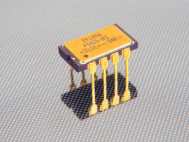
\includegraphics[width=0.15\paperwidth]{img/05/TY1004.png} \\ \hline

        Package: & custom & SOT23-6 & 8-pin ceramic DIL \\ \hline

        \# of transistors: & 2 & 2 & 2 \\  \hline

        Recommended readout current: & $10$ - \SI{500}{\micro\ampere} & \multicolumn{2}{c|}{\SI{10}{\micro\ampere}} \\ \hline

        TID dependency: & $n = 1$, $A~=~0.117$~\si{\milli\volt/\rad} & $n = 0.46$, $A~=~29.5$~\si{\milli\volt/\rad} & $n = 0.41$, $A~=~65.6$~\si{\milli\volt/\rad} \\ \hline
        Temperature readout: & diode & diode & diode \\ \hline
    \end{tabular}
    \end{table}


\section{COTS MOSFET as RadFET}
    RadFETs are specifically designed MOSFETs that act as radiation sensors. However, the parameters of COTS MOSFET transistors also depend on total absorbed dose. They are much cheaper, but require proper calibration and testing in order to be considered as a flight solution.

    Many articles and papers prove that COTS MOSFETs can be used reliably as TID sensors. A number of available transistors were tested, their basic characteristics are compared in the table \ref{cots_mosfet_comparison}. Parameters are taken at unbiased gate.

    \begin{table}[H]
    \caption{COTS MOSFET comparison}
    \label{cots_mosfet_comparison}
    \begin{tabular}{| L{2cm} | C{2.4cm} | C{2.4cm} | C{2.4cm} | C{2.4cm} | C{2.4cm} |}
        \hline
        Type: & 3N163 & ZVP3306 & ZVP4525 & BS250F & CD4007 \\ \hline
        Reference: & \cite{3N163_article} & \cite{COTSMosfetsGarcia} & \cite{COTSMosfetsGarcia} & \cite{COTSMosfetsGarcia} & \cite{COTSMosfetsGarcia} \\ \hline

        Package: & TO-72 & TO-92 & SOT-223 & SOT-23 & TSSOP-14 \\ \hline

        $I_{ZTC}$ [\si{\micro\ampere}]: & 225 & - & - & - & 145 \\ \hline

        Sensitivity [\si{\milli\volt/\gray}]: & $24.3\pm 1.8$ & $3.7\pm 0.3$ & $3.4\pm 0.4$ & $3.1\pm 0.4$ & $4.6\pm 0.1$ \\ \hline

        $V_{TH_0} [\si{\volt}]$: & $2.0 - 3.0$ & $2.0 - 3.0$ & $1.5 - 2.5$ & $2.5 - 3.5$ & $1.9 - 2.5$ \\ \hline

        $V_{TH}$ @ \SI{100}{\gray} [\si{\volt}]: & $5.61$ & $3.4$ & $2.88$ & $3.85$ & $2.97$ \\ \hline
    \end{tabular}
    \end{table}

    3N163 type have the greatest sensitivity - but bearing in mind the \SI{5}{\volt} supply for the sensor, it was discarded for too small range. The second best type is CD4007, which was selected for testing. Its parameters are suitable for the use under discussion, as shown in the table \ref{CD4007_parameters}.

    Other advantages of CD4007 are:
    \begin{itemize}
        \item 3 P-MOS in one package - averaging/redundancy,
        \item additional diodes and transistors in device - possible temperature measurement
        \item small, vibration and thermally resistant package
    \end{itemize}

\section{Selected MOSFET - CD4007}
    The CD4007 consists of three complementary pairs of N- and P-channel enhancement mode MOS transistors. Internal connection diagram is shown below in the figure \ref{CD4007_internal_diagram}. Predicted parameters of those transistors are collected in the table \ref{CD4007_parameters}.

    \begin{figure}[H]
        \centering
        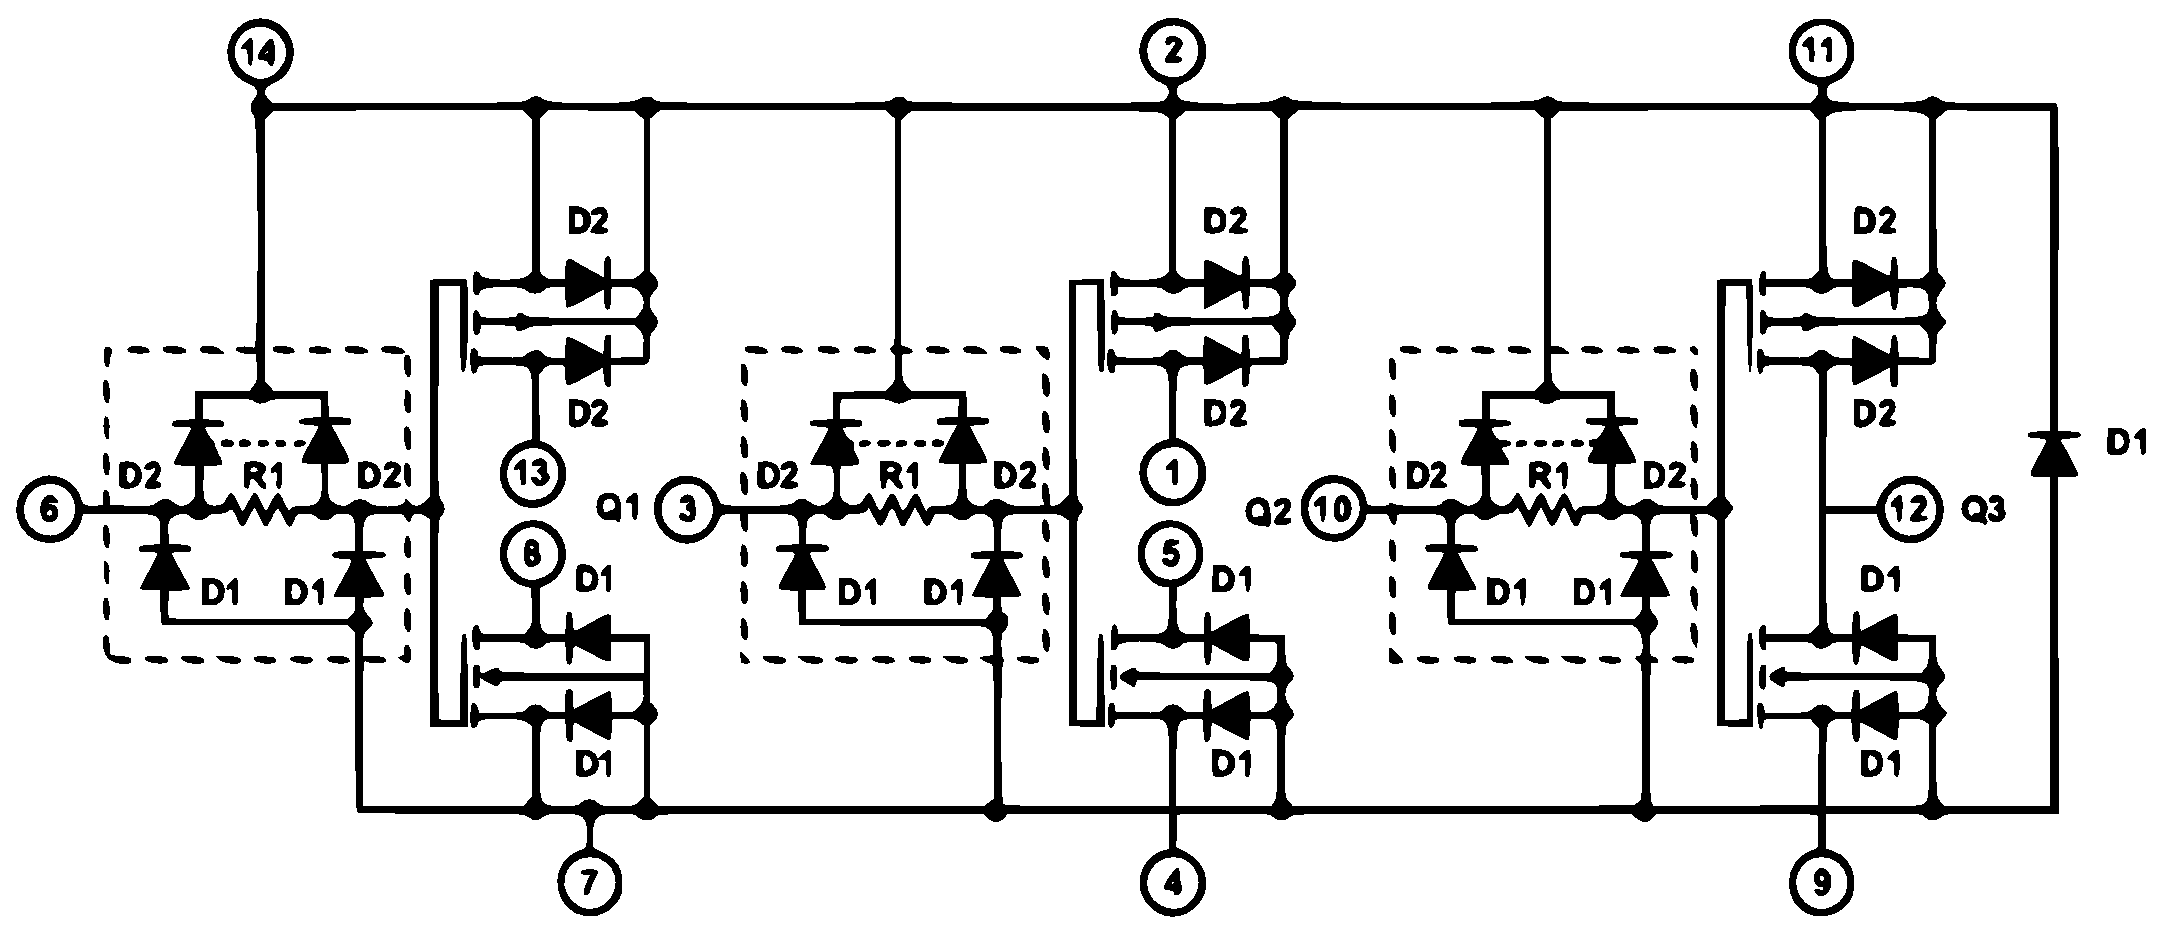
\includegraphics[width=0.7\paperwidth]{img/05/cd4007.eps}
        \caption{CD4007 internal diagram. Source: \cite{CD4007_schematic_functional}}
        \label{CD4007_internal_diagram}
    \end{figure}

    \begin{table}[H]
    \caption{CD4007 parameters}
    \label{CD4007_parameters}
    \begin{tabular}{R{7cm} | L{7cm} }
        Transistor type: & 3x P-MOS and 3x N-MOS \\ \hline
        Supply voltage: & 3-18~\si{\volt} \\ \hline
        Threshold voltage: & \SI{1.8}{\volt} @ \SI{100}{\micro\ampere} \\ \hline
        Temperature range: & \SI{-55}{\degreeCelsius} - \SI{125}{\degreeCelsius} \\ \hline
        Zero-temperature coefficient current: & \SI{140}{\micro\ampere} \\ \hline
        Predicted sensitivity: & \SI{4.6}{\milli\volt/\gray}
    \end{tabular}
    \end{table}

\section{Threshold voltage measurement}
    Threshold voltage changes with TID accumulated. The easiest method to measure change of this parameter is to connect the MOSFET in diode configuration, forcing constant drain current. A block diagram of this method is shown in the figure \ref{Vth_readout_block_diagram}.

    \begin{figure}[H]
        \centering
        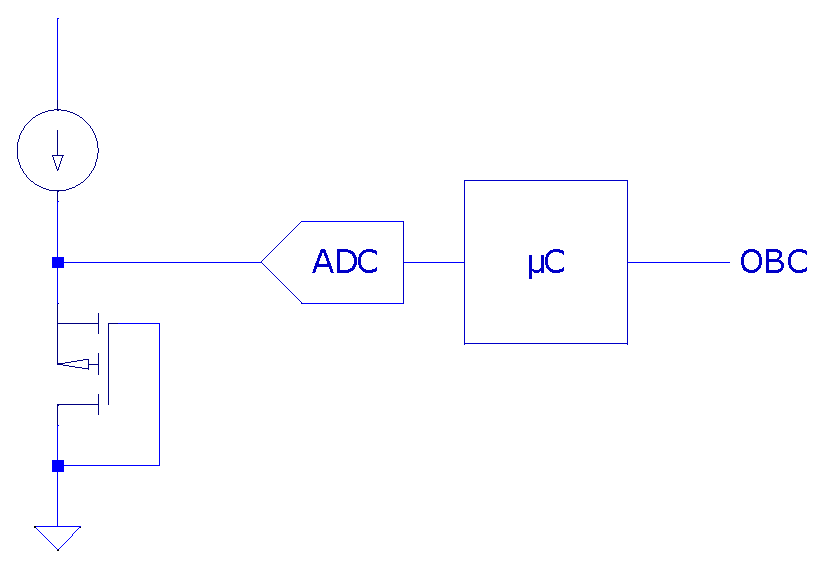
\includegraphics[width=0.3\paperwidth]{img/05/conceptual_block_diagram.eps}
        \caption{Threshold voltage readout block diagram}
        \label{Vth_readout_block_diagram}
    \end{figure}

    In saturation region, drain current is described by the following equation (body effect is negligible):

    $$I_D = A \cdot (V_{GS} - V_{th})^2$$
    Where:

    \begin{tabular}{lcl}
        $I_D$ & - & drain current \\
        $A = \frac{\mu_n C_{ox}}{2} \frac{W}{L}$ & - & constant for partuicular transistor \\
        $V_{GS}$ & - & gate-source voltage \\
        $V_{th}$ & - & threshold voltage \\
    \end{tabular}
    \bigskip

    Because only the threshold voltage change is of interest, measuring $V_{GS}$ has the same effect:
    $$I_D = A \cdot (V_{GS_1} - V_{th_1})^2 = A \cdot (V_{GS_2} - V_{th_2})^2$$
    $$\Delta V_{GS} = \Delta V_{th}$$

    The sensor should be shut down during irradiation - therefore no-bias method was used. It allows for complete isolation of supply power to the sensor, enabling it only for readout.

\section{Temperature measurement}
    Because threshold voltage strongly depends on die temperature, this effect has to be compensated for. The flight MOSFET will be calibrated in a thermal chamber prior to launch, thus obtaining characteristic curves.

    A number of possible temperature measurement techniques were considered during this thesis:
    \begin{table}[H]
    \caption{Temperature readout methods}
    \begin{tabular}{C{4.5cm} | C{5cm} | C{5cm} }
        \textbf{Method} & \textbf{Pros} & \textbf{Cons} \\ \hline

        PT-1000 sensor glued to MOSFET & accurate reading & large thermal resistance, difficult assembly, low reliability \\ \hline

        ESD diode measurement in CD4007 & no additional sensor & complicated current, multiplexing circuit, unknown characteristics \\ \hline

        body diode in N-MOSFET in CD4007  & simple setup, reliable, known characteristics, low thermal resistance & no possibility of simultaneous readout of threshold and temperature (short thermal lag)
    \end{tabular}
    \end{table}

    The chosen solution: to measure temperature of silicon die using body diode in complementary N-MOS transistor. A block diagram of this proposed solution is presented in the figure \ref{Temperature_measurement_block_diagram}.

    \begin{figure}[H]
        \centering
        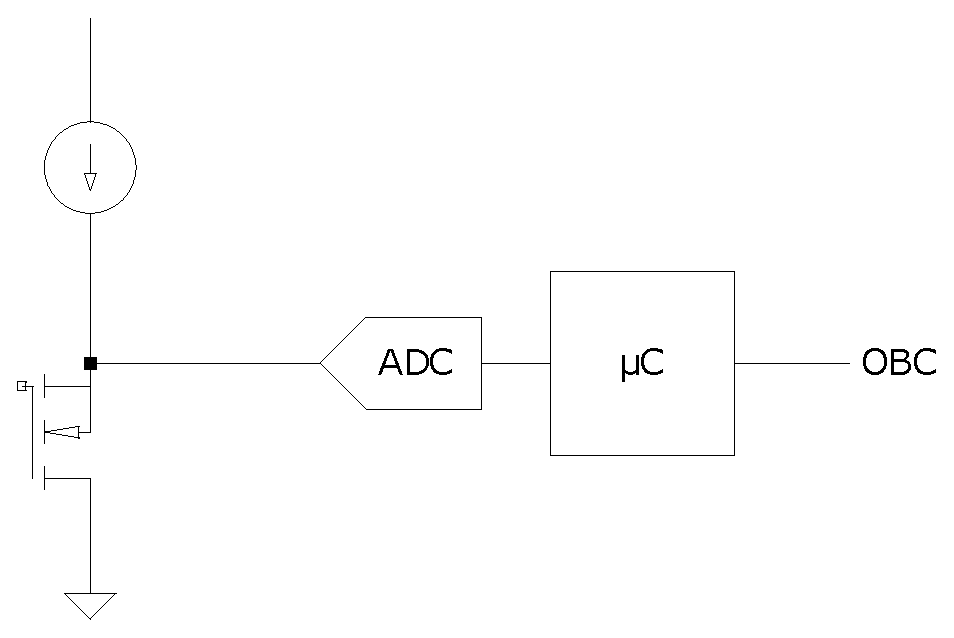
\includegraphics[width=0.5\paperwidth]{img/05/n-mos-temperature.eps}
        \caption{Temperature measurement block diagram}
        \label{Temperature_measurement_block_diagram}
    \end{figure}

    During calibration, both the temperature characteristics of the diode and the p-MOS threshold voltage will be obtained. They will be used to compensate for the threshold voltage shift associated with temperature. An individual flight component will be placed in a thermal chamber, and a proper look-up table will be created, with possible polynomial approximation.

\newpage
\section{Characteristic curves}
\label{Characteristic_curves}

    During M. Gumiela's thesis, \cite{MGThesis} a calibration stand for CD4007 was developed. As an outcome of that project, rough calibration curves were obtained, which are presented below.

    \bigskip \textbf{p-MOSFET transfer characteristics}
    \begin{figure}[H]
        \centering
        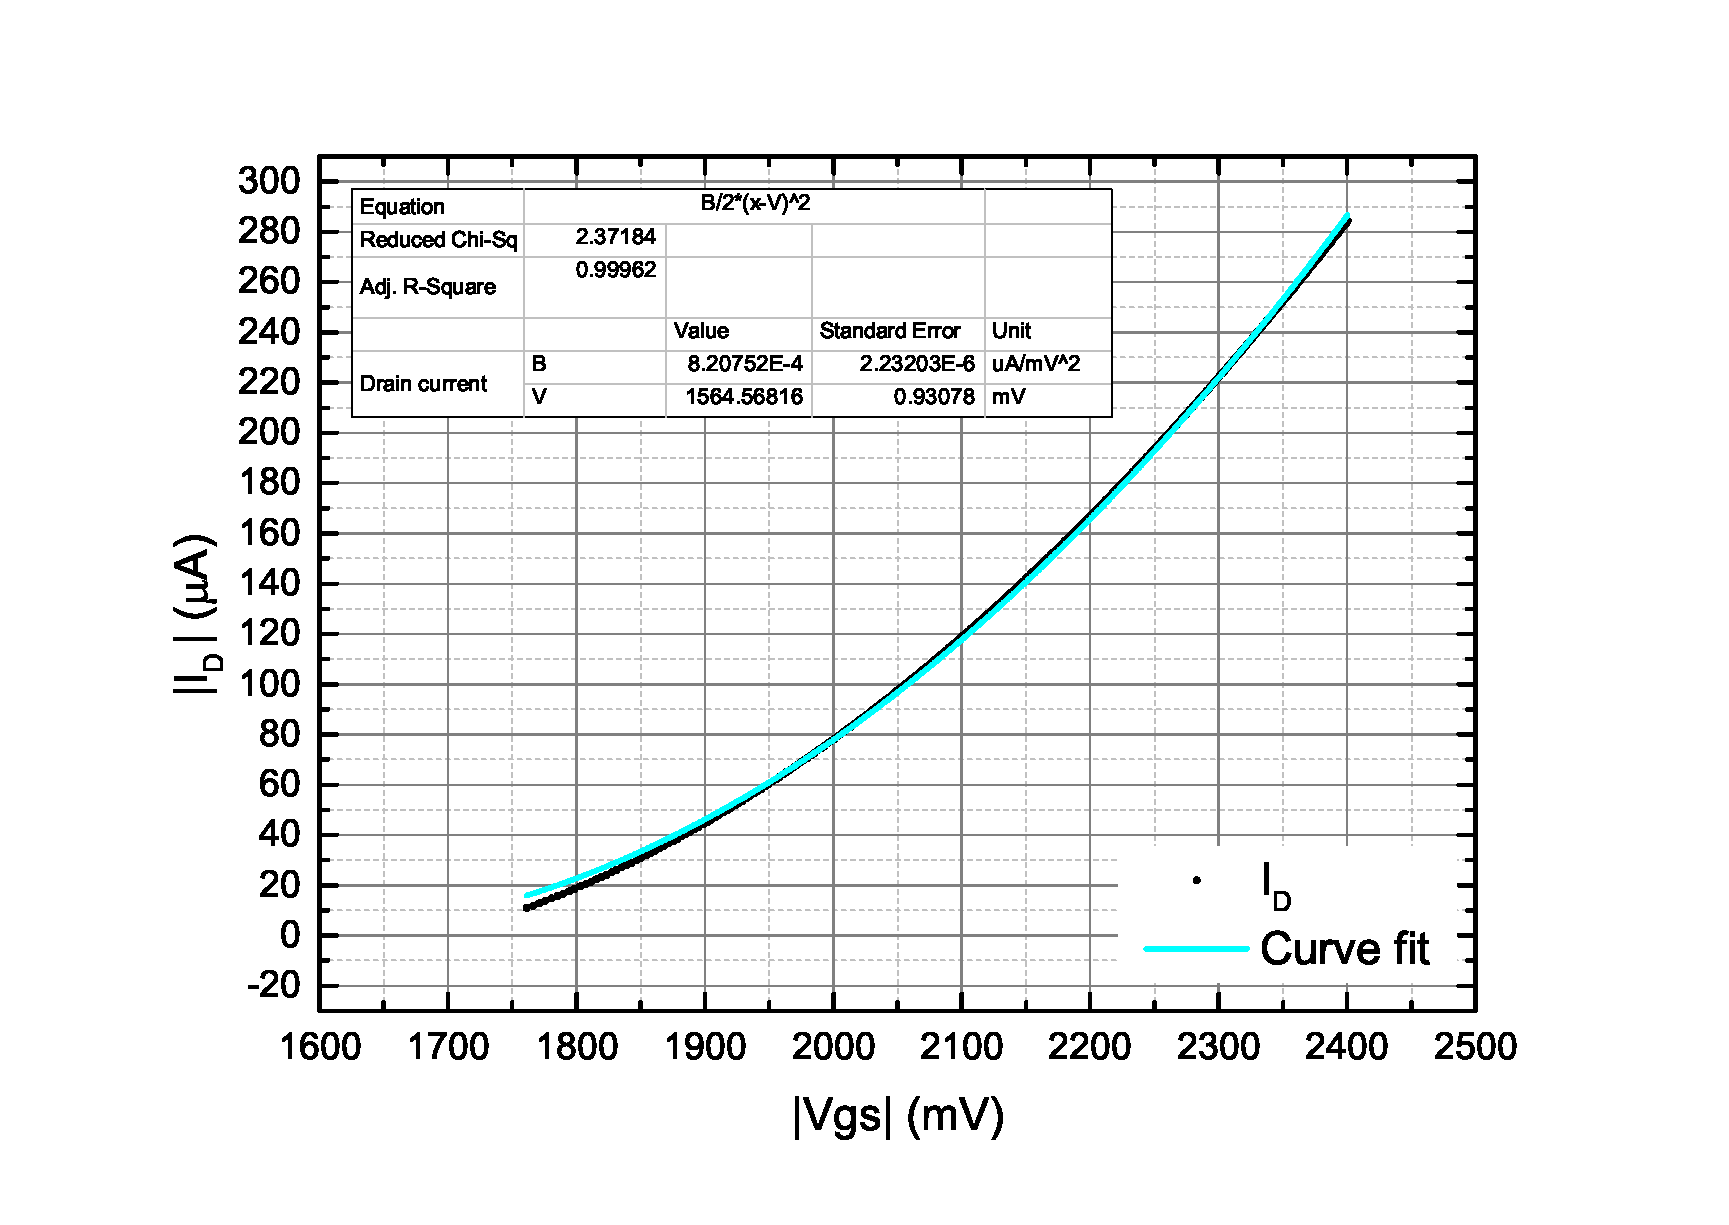
\includegraphics[width=0.56\paperwidth]{img/05/mg_iv_mosfet.eps}
        \caption{CD4007 p-MOSFET transfer characteristics. Source: \cite{MGThesis}}
        \label{CD4007_p-MOSFET_transfer}
    \end{figure}

    \bigskip \textbf{Linearized temperature coefficient of threshold voltage}
    \begin{figure}[H]
        \centering
        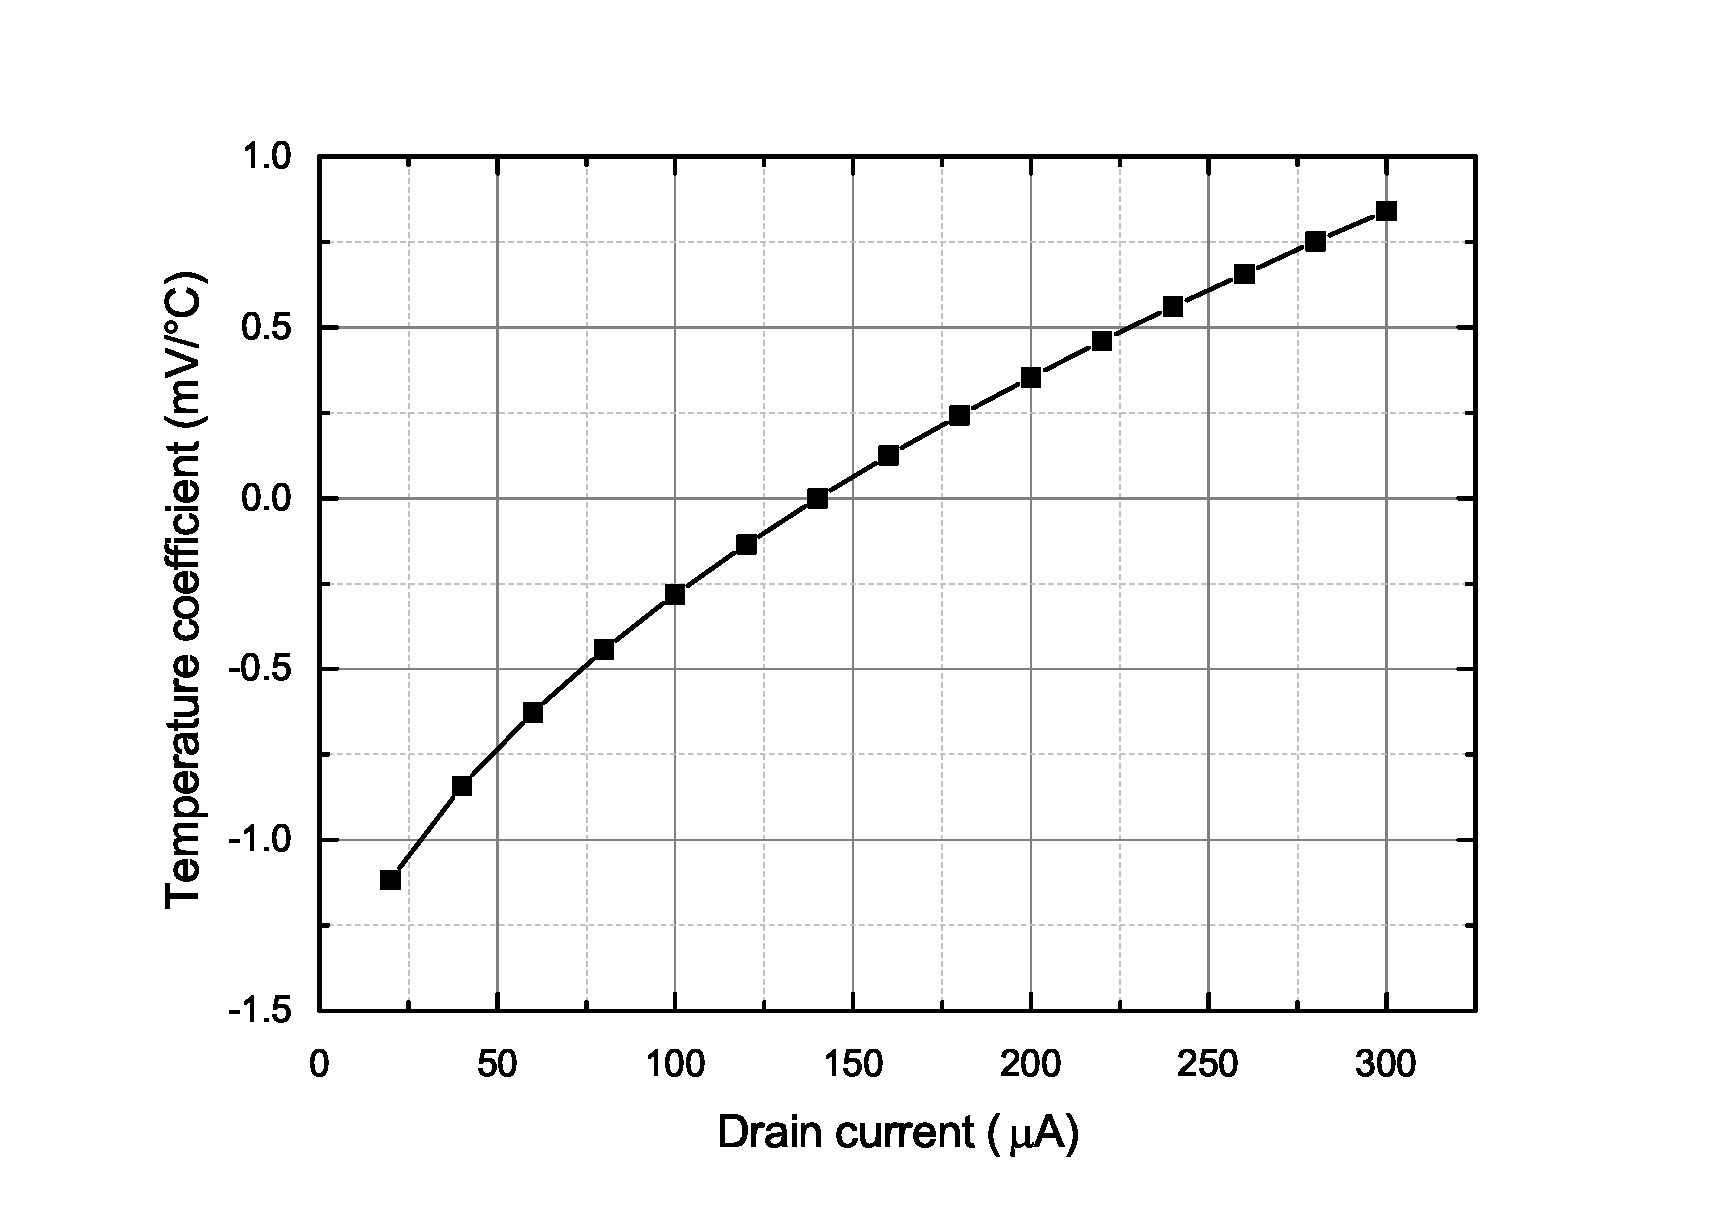
\includegraphics[width=0.56\paperwidth]{img/05/mg_tc_coefficients.eps}
        \caption{Linearized temperature coefficient of threshold voltage. Source: \cite{MGThesis}}
    \end{figure}

    \bigskip \textbf{Body diode forward voltage temperature calibration}
    \begin{figure}[H]
        \centering
        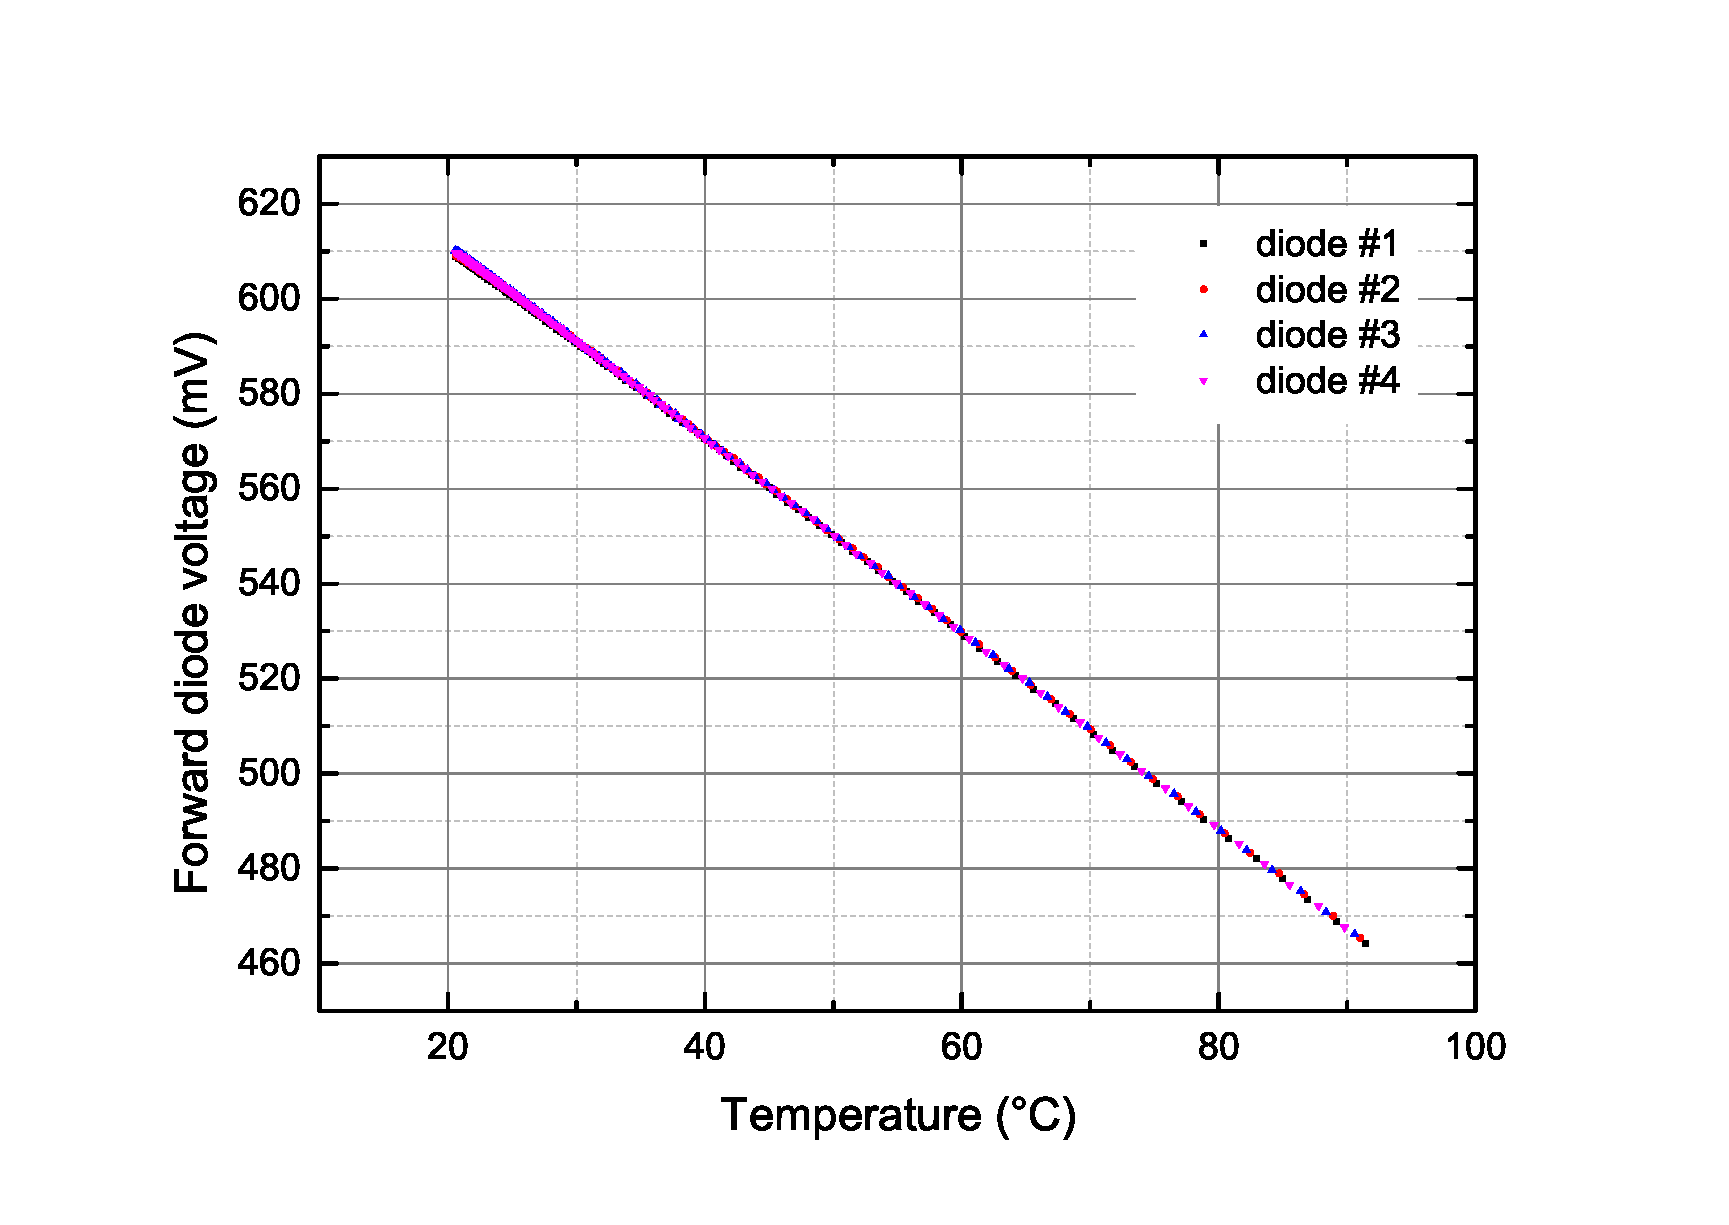
\includegraphics[width=0.7\paperwidth]{img/05/mg_diode_temp.eps}
        \caption{Body diode temperature calibration. Source: \cite{MGThesis}}
    \end{figure}

\section{Operating point selection}
    A current source value had to be chosen, keeping in mind the requirements and working conditions.

    In theory, a zero-temperature coefficient current would be optimal, but after irradiation it could shift slightly, causing a significant error. Additionally, due to limited availability of elements on the market and slight differences between devices, this operating point would be very difficult to achieve.

    As a tradeoff between low temperature coefficient and low starting threshold voltage, (to increase sensor range) the current value of \SI{125}{\micro\ampere} was chosen.

% Sensor design
% - Commercial RadFETs
% - MOSFET as RadFET
% - Chosen MOSFET: CD4007
% - Conceptual Block diagram
% - Characteristic curves (MG)
% - Operating point selection

\chapter{Sensor prototypes}

\section{Demonstration model}
\section{Calibration stand}
% Sensor prototypes
% - Demonstration model
% - Calibration stand

\chapter{Engineering model}

\section{Block diagram}

\section{Low-level requirements}

\section{Analog front-end}
\subsection{Current source}
\subsection{ADC}
\subsection{Multiplexer}
\subsection{LDO}
\subsection{Shielding}

\section{Digital}
\subsection{Microcontroller}
\subsection{OBC interface}

\section{Software design}
\subsection{AVR-HAL}
\subsection{I2C-slave module}
\subsection{Measurement algorithm}

\section{PCB}
\subsection{PCB stack}
\subsection{PCB layout}
\subsection{3D model}
\subsection{Manufacturing}

\section{Assembly}

\section{Finished sensor}

% Engineering model
% - Block diagram
% - Low-level requirements
% - Analog front-end
% -- Current source
% -- ADC
% -- Multiplexer
% -- LDO
% -- Shielding
% - Digital
% -- Microcontroller
% -- OBC interface
% - Software design
% -- AVR-HAL
% -- I2C-slave module
% -- Measurement algorithm
% - PCB
% -- PCB stack
% -- PCB layout
% -- 3D model
% -- Manufacturing
% - Assembly
% - Finished sensor

\chapter{Sensor tests}

\section{Digital}
\subsection{Interface tests}
\subsection{Software tests}

\section{Analog}
\subsection{Measurement noise}
\subsection{Temperature stability}
\subsection{Ageing stability}
\subsection{Irradiation tests}

% Sensor tests
% - Digital
% -- Interface tests
% -- Software tests
% - Analog
% -- Measurement noise
% -- Temperature stability
% -- Ageing stability
% -- Irradiation tests

\chapter{Flight model}

% Flight model

\chapter{Summary}

% Summary
%
% Figures
% Tables



\appendix
\printbibliography

\end{document}
